%!TEX root = ../my_thesis.tex

\chapter{Contexte et état de l'art}
Ce premier chapitre expose les concepts de base du codage canal ainsi que les turbo codes.

Dans la première section, les notions essentielles des codes correcteurs d'erreurs sont présentées. Elles couvrent la notion d'information dans le cadre des télécommunications, la théorie de l'information de Claude Shannon et une présentation de quelques codes correcteurs élémentaires.

Dans la seconde section, les turbo codes convolutifs sont ensuite définis. D'abord, leur construction, puis leur décodage. Les performances des turbo codes standardisés sont succinctement exposées. Ceci amène la prédiction des performances asymptotiques des turbo codes. Finalement, différentes méthodes permettant d'améliorer les performances des turbo codes standardisés sont décrites. 

\vspace*{\fill}
\minitocTITI
\vspace*{\fill}

\section{Définitions et fondamentaux}

\subsection{Introduction}
\og Le problème fondamental de la communication est de reproduire à un endroit donné de manière exacte ou approximative 
un message sélectionné à un autre endroit.\fg

Voilà ce qu'écrivit Claude Shannon dans son papier "A mathematical Theory of Communication" \cite{shannon_mathematical_2001}, 
paru en 1948 alors qu'il exerçait en tant qu'ingénieur au sein des laboratoires Bell. Ses travaux prennent notamment 
leurs sources dans les publications de Harry Nyquist \cite{nyquist_telegraph} et Ralph Hartley \cite{hartley_trans}, 
chercheurs eux aussi auprès des laboratoires Bell alors qu'ils visent à augmenter la vitesse de transmission des signaux sur 
les lignes de télégraphe. 

Hartley est sans doute le premier à employer le mot d'information dans un contexte technique ou scientifique. Cette 
quantité mesurable reflète alors la capacité d'un récepteur à distinguer un message émis par une 
source plutôt qu'un autre.

En posant deux théorèmes fondamentaux, les travaux de Claude Shannon permettent d'ouvrir la voie à la théorie de 
l'information. Tout d'abord, ils dressent le modèle d'une communication, connu aussi sous le nom de 
\emph{paradigme de Shannon} dans lequel une source génère un message pour un destinataire. La source et le 
destinataire sont séparés par un canal, média de transmission du message. 
%Ce média est caractérisé par un phénomène de propagation (qui permet au message d'atteindre le destinataire) et par un phénomène de perturbation (qui dégrade le message transmis). 
Ce média est caractérisé par un phénomène de propagation et par un phénomène de perturbation. Le premier permet au message d'atteindre le destinataire alors que le second dégrade le message transmis.

\begin{figure}[!h]
	\centering
	\includegraphics[width=10cm]{main/ch1_fig/shParadigm.pdf}
	\caption{\label{fig:paradigme} Schéma simplifié d'une communication}
\end{figure}


Les deux théorèmes fondamentaux de Shannon définissent deux limites théoriques. L'une, quant au codage de source, 
consiste à obtenir le maximum de concision dans l'expression d'un message, mais n'est pas traité dans ce manuscrit. 
L'autre limite concerne le codage canal qui vise à rendre robuste un message face aux perturbations du canal et est au cœur de ces travaux de thèse. Avant de détailler ce second principe, il est nécessaire de définir la mesure de l'information.
%---------------------------------------%
\subsection{La mesure de l'information}
\subsubsection{Variable aléatoire}
\paragraph*{Information propre}
Soit $X$ une variable aléatoire dont les réalisations appartiennent à l'ensemble fini $\mathcal{X}$. L'observation de 
l'événement $X=x$, avec $x\in \mathcal{X}$, a pour probabilité $p$. La quantité d'information associée à la réalisation
de cet événement est définie par \[h(x)=-\log(p).\]
La base du logarithme fixe l'unité de la mesure de l'information. Habituellement la base 2 est
choisie et l'unité est le \emph{bit}. Néanmoins ce nom peut prêter à confusion avec le chiffre du système binaire. 
Ainsi, le système international \cite{ISO} définit le \emph{shannon} (Sh) comme l'unité dé mesure de l'information. Un shannon 
représente la quantité d’information associée à la réalisation d'un des deux événements équiprobables qui s’excluent 
mutuellement. 

Qualitativement, fournir une information est équivalent à lever une incertitude. Ainsi, plus un événement est imprévu, 
plus il apporte de l'information.

\paragraph*{Entropie}
La valeur moyenne de l'information propre calculée sur la totalité de l'ensemble $\mathcal{X}$ est appelée entropie (ou 
incertitude) de la variable aléatoire $X$ et est notée $H(X)$. Soit $n$ le cardinal de $\mathcal{X}$ et $p_i$ la 
probabilité que l'événement $X=x_i$ se réalise avec $i\in \llbracket 1; n\rrbracket$, alors, 
\[H(X) = \sum\limits_{i=1}^n p_i\times h(x_i) = - \sum\limits_{i=1}^n p_i\times log(p_i).\]

L'entropie correspond à la quantité d'information délivrée par une source. Elle est exprimée en shannon 
par symbole, les symboles étant les réalisations possibles de cette source. L'entropie d'une source est toujours positive
ou nulle. Sa valeur est maximale lorsque les symboles à la sortie de la source sont équiprobables.

\subsubsection{Couple de variables aléatoires}
Considérons maintenant une deuxième variable aléatoire $Y$ dont les réalisations appartiennent à l'ensemble fini $\mathcal{Y}$, avec 
$m=\card(\mathcal{Y})$.
\paragraph*{Entropie conjointe}
En étendant la définition précédente, l'entropie conjointe de deux variables aléatoires est définie par : 
\[H(X, Y) = - \sum\limits_{i=1}^n\sum\limits_{j=1}^m P(X=x_i, Y=y_j) \log P(X=x_i, Y=y_j).\]
Elle mesure la quantité moyenne d'information contenue dans un système de deux variables aléatoires. 
Ainsi, naturellement, $H(X, Y) \geq \max \left[H(X), H(Y)\right]$.
\paragraph*{Entropie conditionnelle} 
$H(X|Y=y_j)$ est l'entropie de la variable $X$ sachant que la variable $Y$ prend la valeur $y_j$ et est définie par :
\[H(X|Y=y_j) = - \sum \limits_{i=1}^n P(X=x_i|Y=y_j)\log P(X=x_i|Y=y_j)\]
En calculant la moyenne de $H(X|Y=y_j)$ pour tout $y_j\in \mathcal{Y}$ est obtenue l'entropie conditionnelle de $X$ sachant $Y$ : 
\[H(X|Y) = \sum\limits_{j=1}^m P(Y=y_j) H(X|Y=y_j).\] Elle décrit l'incertitude restante sur la variable aléatoire $X$ 
lorsque la variable aléatoire $Y$ est connue.
\paragraph*{Information mutuelle}
L’information mutuelle mesure la quantité d'information partagée entre $X$ et $Y$. En d'autres termes, elle mesure la 
dépendance entre ces deux variables. Ainsi, l'information mutuelle est nulle si et seulement si les variables sont 
indépendantes et elle croît lorsque leur degré de dépendance augmente.
\[I(X;Y) = \sum\limits_{i=1}^n\sum\limits_{j=1}^m P(X=x_i,Y=y_j) \log\left(\frac{P(X=x_i, Y=y_j)}{P(X=x_i)P(Y=y_j)}\right),\]
L'expression de l'information mutuelle peut être formulée en utilisant l'entropie conditionnelle
\begin{equation}
	I(X;Y) = H(X) - H(X|Y).
	\label{eq:imut}
\end{equation}
%---------------------------------------%
\subsection{Le codage canal}
Dans le cadre de ce manuscrit, seuls sont considérés des canaux de transmission causaux sans effet mémoire et stationnaires. En d'autres termes, la sortie du canal à l'instant $t$ ne dépend que de son entrée en l'instant $t$.\\
Considérons maintenant que $X$ soit la variable aléatoire à l'entrée du canal et $Y$ la variable aléatoire à sa sortie.
\subsubsection{Capacité d'un canal}
Par définition, la capacité du canal est l'information mutuelle maximale entre $X$ et $Y$ : \\
$C=\sup\limits_{\underline{p}}\ I(X;Y)$, avec $\underline{p}$ la distribution de probabilité des symboles à l'entrée 
du canal. La capacité représente la quantité d'information maximale que le canal peut transporter et son unité est le 
shannon par symbole.

D'après l'équation \ref{eq:imut}, afin d'obtenir une communication efficace, il est nécessaire que $H(X|Y)$ soit aussi
petit que possible. Or, ce terme, dépend du canal. Plus le canal est bruité, plus ce terme est grand. Le message 
source doit alors être modifié pour que la communication satisfasse une contrainte de qualité. Ceci constitue le codage 
canal. Son principe est d'ajouter de la redondance en quantité suffisante pour éviter toute ambiguïté lors du décodage.

\subsubsection{Le théorème du codage canal}
Le second théorème de Shannon énonce : quel que soit $\epsilon > 0$, il existe un code de taille $N$, avec $N$ \
suffisamment grand, tel que si $R<C$ -- avec R le rendement du code et $C$ la capacité du canal -- la probabilité
d'erreur après décodage soit inférieure à $\epsilon$. 

Ce théorème fournit donc une mesure de la performance d'un système de communication. Un système atteignant la capacité 
du canal peut être considéré comme optimal. Dès lors, le but du codage canal est de définir des codes permettant de 
s'approcher au plus près de cette limite théorique tout en assurant un décodage relativement simple.

Ainsi, le schéma présenté en Figure \ref{fig:paradigme} se doit d'être modifié en prenant en compte ce codage. Aussi,
afin de rendre possible la propagation de l'information à travers le canal, il est nécessaire de mettre en forme le flux 
de données. Par exemple, dans le cas d'une communication sans fil, ce flux doit être représenté par un signal haute 
fréquence afin de pouvoir être émis par une antenne de taille raisonnable. Ceci est le rôle du modulateur.
La Figure \ref{fig:paradigme2} présente une chaîne de communication numérique classique prenant en compte ces deux
nouveaux éléments.
\begin{figure}[!h]
	\centering
	\includegraphics[width=12cm]{main/ch1_fig/shParadigm2.pdf}
	\caption{\label{fig:paradigme2} Schéma fondamental de communication (ou paradigme de Shannon)}
\end{figure}

La source génère un flux de bits $\mathbf{m}$ qui constitue le message à envoyer. Le codeur canal transforme ce message 
en un mot de code $\mathbf{c}$. Ceci est fait en ajoutant de la redondance au message. Ainsi, $H(m)>H(c)$. Le rapport $R$
entre la taille du mot présent à l'entrée de l'encodeur et la taille du mot codé est appelé le rendement du code. Le mot de code est ensuite mis en forme par le modulateur afin d'être transmis via le canal.\\
La chaîne de réception est le dual de la chaîne d’émission. Le démodulateur traite la forme d'onde reçue du canal 
pour transmettre les symboles bruités au décodeur. Si la sortie du démodulateur consiste en une suite binaire, le 
décodage est dit à \emph{entrées dures}. Si par contre, la sortie du filtre adapté est directement passée au décodeur, 
le décodage est dit à \emph{entrées pondérées}. Le décodeur, se servant de la séquence reçue et de la connaissance des règles 
d'encodage fournit une estimation sur le  mot transmis le plus probable $\mathbf{\hat{m}}$.


\subsubsection{Le modèle du canal}\label{ss:cod_canal}
Afin de décrire les perturbations subies par le message transitant à travers le canal de transmission, différents modèles 
peuvent être utilisés. 
%Dans ce mémoire le canal additif à bruit blanc Gaussien à entrée binaire (BI-AWGN) est considéré. 
%Les modulations employés seront par changement de phase (PSK). Pour l'instant, uniquement la la modulation par 
%changement de phase binaire est employé (BPSK). Dans ce cas, chaque bit du mot de code est translaté sur $\{-1;1\}$.
Cependant, le choix du modèle se porte très souvent dans la littérature sur le canal à bruit additif blanc Gaussien 
(AWGN). 
Ce canal modélise notamment très bien le bruit thermique qui est une des sources de bruit toujours présente du côté du récepteur.
%Certes, ce canal n'est pas un modèle très fin quant à la quali mais permet tout de même de comparer de manière
%juste différents schémas de codage.

La loi liant la sortie $y_i$ d'un canal AWGN à son entrée $x_i$ est de la forme $y_i=x_i+n_i$ avec $n_i$ une variable 
indépendante et identiquement distribuée suivant une loi normale (ou gaussienne) centrée en zéro et de variance $\sigma^2 = \frac{N_0}{2}$. Nous avons donc
$N_i \sim \mathcal{N}(0,\ \sigma^2)$ et il vient :
%La densité de probabilité de N est alors : $p(Z) = \frac{1}{\sqrt{2\pi \sigma^2}}\cdot \exp(-{\frac{Z^2}{2\sigma^2}})$
%et donc
\begin{equation}
	\label{eq:p(y|x)}
	P(y_i|x_i) = \frac{1}{\sqrt{2\pi \sigma^2}}~\exp\left(-{\frac{(y_i-x_i)^2}{2\sigma^2}}\right)
\end{equation}

\paragraph*{Capacité du canal AWGN}
À partir de l'équation \ref{eq:imut} et de la densité de probabilité du bruit exprimé par l'équation \ref{eq:p(y|x)}, la capacité du canal 
AWGN est donnée par \begin{equation}\label{eq:capacity}
C = \frac{1}{2} \log_2\left(1 + \frac{P}{\sigma^2}\right),
\end{equation}
exprimé en shannon par symbole émis, avec P la puissance du signal émis.

%---------------------------------------%
\subsection{Les familles de codes correcteurs}
Les codes correcteurs d'erreur largement utilisés dans les différents standards de communications numériques 
appartiennent à deux familles distinctes. Il s'agit des codes en blocs linéaires et des codes convolutifs. Par définition, 
les codes convolutifs vont pouvoir traiter des flots continus de données alors que des codes en blocs permettent 
de traiter des blocs de données indépendants.
\subsubsection{Codes en blocs linéaires}
Historiquement, les premiers codes correcteurs d'erreurs découverts furent les codes en blocs linéaires. La théorie 
mathématique les définissant est basée sur les corps de Galois. Dans la suite, la majorité des opérations se dérouleront 
dans le corps de Galois à 2 éléments noté $GF_2$.
\paragraph*{Définition}
Un code en bloc est une application $g$ de $GF_2^k$ dans $GF_2^n$, avec $k<n$, qui à un vecteur $m$ de taille $k$ associe
un autre vecteur $c$ de taille $n$. Les $2^k$ éléments $c$ sont appelés mots de code. Le rapport $k/n$  est appelé le 
rendement du code. Le nombre d'éléments binaires de redondance ajoutés est donné par $k-n$. Si $g$ est linéaire, alors 
il s'agit d'un code en bloc linéaire. Il existe alors un matrice $G$ à $k$ lignes et $n$ colonnes associée à 
l'application $g$. Elle est appelée matrice génératrice du code $C(n,k)$. \\
Aussi, nous pouvons définir $H$, la matrice génératrice du dual du code $C(n,k)$. Ainsi, pour tout mot de code $c$ de 
$C(n,k)$, nous avons : \[cH^t = 0.\]
Si $G$ peut s'écrire de la forme $G=[I_k,P]$ avec $I_k$ la matrice identité de taille $k$, alors  le code $C(n,k)$ est dit
\emph{systématique}.
\paragraph*{Détection d'erreur}
Avant d'évoquer le principe de décodage, il est nécessaire de présenter celui de la détection d'erreur. Supposons que 
nous codons un message $m$ de taille $k$ par un code en bloc linaire $C(n,k)$, tel que $c = mG$. Si ce message est 
transmis sur un canal bruité sans effet mémoire, le démodulateur à décision dure fournit au décodeur le vecteur $r$, de 
taille $n$ représentant le mot reçu. Celui-ci peut s'écrire de la forme \[r=c+e\] avec $e$
un vecteur ligne dont les composantes binaires correspondent aux éventuelles erreurs de transmission. La détection 
d'erreur se fait alors en calculant le \emph{syndrome} : \[s = rH^t = (c+e)H^t = eH^t.\]
$s=0$ si et seulement si $r$  est un mot du code. Si $s \ne 0$, alors il existe des erreurs de transmission. La 
réciproque n'est pas vraie car la combinaison linéaire de deux mots de code est aussi un mot du code. Il s'agit de la conséquence directe de la linéarité de $g$.
\paragraph*{Principe du décodage}
Il est possible de définir une distance entre deux mots de code, appelée \emph{distance de Hamming ($d_H(c, c')$)}. 
Définissons tout d'abord le poids de Hamming d'un mot de code ($P_H(c)$) comme étant le nombre de ses éléments non nul. 
La distance de Hamming entre deux mots de codes est égale au poids de Hamming de leur combinaison linéaire : 
$d_H(c, c') = P_H(c+c')$.

Le principe du décodage par maximum de vraisemblance consiste en la recherche du mot de code $\hat{c}$ le plus 
vraisemblable, c'est à dire celui qui est à la distance de Hamming minimale du mot de code reçu $r$. C'est à dire trouver 
$\hat{c}$, tel que \[d_H(r,\hat{c}) \leq d_H(r,\hat{c}) \forall c \neq \hat{c} \in C.\]

Il vient donc assez naturellement que les performances de décodage d'un code sont dépendantes des distances de Hamming 
séparant les différents mots de code. La valeur minimale de cet ensemble de distances est appelée \emph{la distance minimale du code}, 
notée $d_{min}$. \[d_{min}=\min\limits_{c,c'\in C}d_h(c, c').\] Comme le code est linéaire, la distance minimale 
est aussi égale au poids minimal des mots de code non nuls. Ainsi, le poids des mots de code (excepté le mot 
de code nul) est compris entre $d_{min}$ et $n$. Le nombre de mots de code de poids de Hamming $d$ est appelé 
\emph{multiplicité} et est noté $A_d$.

\paragraph*{Codes cycliques} Un code en bloc linéaire est dit cyclique si la permutation circulaire vers la 
gauche d'un mot de code est aussi un mot de code. C'est-à-dire que si $c = \{c_0, ..., c_j, ..., c_{n-1}\}$ est un mot 
de code, $c' = \{c_1, ..., c_j, ..., c_{n-1}, c_0\}$ est aussi un mot de code.

Ces codes sont souvent représentés sous forme polynomiale. Or, en électronique numérique, une division polynomiale est aisément 
réalisable à partir de registres à décalage. Ils ont donc été particulièrement étudiés et sont présents aujourd'hui dans 
de nombreux standards de communication numériques. Nous pouvons par exemple citer les codes BCH du nom de leurs inventeurs Bose, 
Ray-Chaudhuri et Hocquenghem \cite{bose1960class}. Ils ont la particularité de pouvoir être construits en fonction du pouvoir 
de correction visé.

Une autre catégorie de codes cycliques est largement utilisée dans les standards de communication actuels. Il s'agit des codes à redondance cyclique (CRC) \cite{crc} qui possèdent un fort pouvoir de détection d'erreurs.

%---------------------------------------%
\subsubsection{Codes convolutifs}
\paragraph*{Définition}
Les codes convolutifs ont été proposés par Peter Elias en 1955 comme une alternative aux codes en blocs \cite{elias}. 
Elias cherche alors à définir un code à longueur variable. Le codage est fait de telle sorte que la sortie dépende de 
l'entrée courante mais aussi des entrées précédentes. Un codeur convolutif peut être vu comme un filtre. La sortie 
est alors le produit de convolution entre l'entrée et la réponse impulsionnelle du codeur. 

En utilisant la notation de Forney de l'opérateur de retard D \cite{forney1970convolutional}, le message peut être exprimé 
sous la forme $m=\sum_k m_kD^k$. De la même manière, le mot codé devient $c=\sum_n c_nD^n$. L'exposant de D représente 
alors l'instant auquel $m_k$ et $c_k$ apparaissent à l'entrée et à la sortie du codeur, respectivement. $c_k$ peut aussi 
être exprimé comme une combinaison linéaire des $\nu$ précédents éléments du message : $c_k = \sum\limits_{j=0}^\nu g_jm_{k-j}$.
La suite d'éléments $g_j$ est appelée séquence génératrice du code. Elle est souvent exprimée en base octale. $\nu$ représente le 
nombre d'éléments de mémorisation à l'intérieur du codeur.

\paragraph*{Exemple}
Soit le codeur convolutif de rendement $R=1/2$, de mémoire $\nu = 2$ présenté en Figure \ref{fig:encConv}. Ses deux 
séquences génératrices définissant les sorties $c_1$ et $c_2$ sont respectivement $G_1 = (5)_8$ et $G_2 = (7)_8$.
\begin{figure}[!h]
	\centering
	\includegraphics[width=6cm]{main/ch1_fig/encConv.pdf}
	\caption{\label{fig:encConv} Exemple de codeur convolutif}
\end{figure}
Puisque $\nu = 2$, ce codeur peut être dans $2^\nu$ états différents. Ainsi, un codeur convolutif peut être vu comme une 
machine de Mealy. Ce diagramme d'états, comme présenté en Figure \ref{fig:stateMachine}, présente les  $2^{\nu+1}$ 
différentes transitions entre les $2^{\nu+1}$ états internes. 
\begin{figure}[!h]
	\centering
	\includegraphics[width=5cm]{main/ch1_fig/stateMachine.pdf}
	\caption{\label{fig:stateMachine} Machine d'états associée au codeur convolutif de la Figure \ref{fig:encConv}}
\end{figure}

\paragraph*{Représentation en treillis}
Néanmoins, la représentation sous la forme d'une machine d'états, bien qu'elle permette de se rendre compte aisément du fonctionnement du 
codeur, ne présente pas d’intérêt pour le décodage. C'est pourquoi, une représentation sous forme de treillis est privilégiée. Elle a
été utilisée pour la première fois par Forney en 1973 \cite{forney73viterbi}. Cette
représentation permet de rendre compte à la fois de l'état interne du codeur, des transitions et de l'évolution 
temporelle. La Figure \ref{fig:trellis} présente le diagramme en treillis associé au codeur convolutif de la Figure 
\ref{fig:encConv}, en considérant que l'état interne du codeur est $S_0$. Comme il n'y a qu'une entrée, de chaque nœud 
partent 2 branches et vers chaque nœud convergent 2 branches. Au bout de $\nu+1$ unités de temps, quel que soit l'état 
initial, le motif du treillis se répète. Cette durée est appelée longueur de contrainte du code convolutif. Lors du 
codage d'une séquence, la connexion entre les différents nœuds est nommée chemin dans le treillis. Sur la Figure  
\ref{fig:trellis} sont présentées sur les branches les 8 associations entrées/sorties possibles.
\begin{figure}[!h]
	\centering
	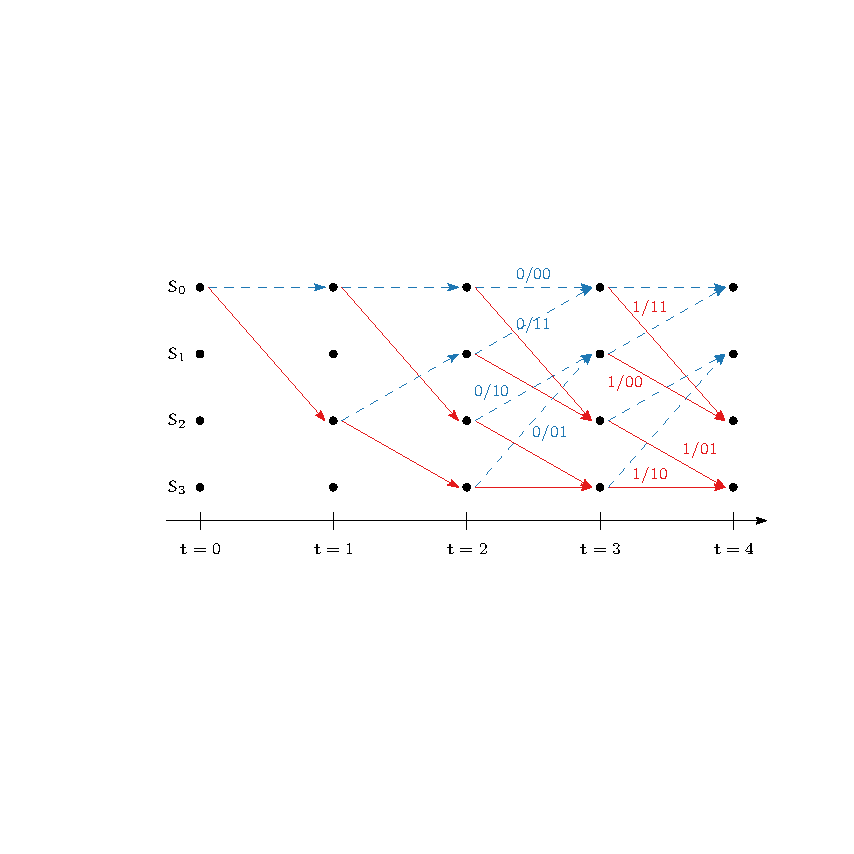
\includegraphics[width=10cm]{main/ch1_fig/trellis.pdf}
	\caption{\label{fig:trellis} Diagramme en treillis du codeur convolutif de la Figure \ref{fig:encConv}}
\end{figure}

\paragraph*{Terminaison}\label{par:term}
Comme évoqué précédemment, l'un des intérêts des codeurs convolutifs est de permettre d'obtenir des mots de codes de 
taille infinie. Néanmoins, dans le contexte de protocoles de communications numériques, les messages ont une taille 
prédéfinie. C'est pourquoi la fermeture du treillis est nécessaire de part son impact non négligeable sur les performances de 
décodage. Trois solutions de terminaison sont à considérer et ont été proposés dans la littérature :
\begin{itemize}
	\item pas de terminaison. L'état final ne peut donc être connu par le décodeur. Ainsi, les derniers symboles encodés
	      sont moins bien protégés. 
	\item forcer l'encodeur à finir dans un état connu. 
	      %Après avoir codé les K bits d'informations, une séquence y est concaténée. 
	      Quel que soit l'état interne du codeur après que les K bits d'information aient été codés, un retour dans n'importe quel état est possible en y ajoutant $\nu$ bits supplémentaires. Le message transmis est alors composé de la séquence initiale concaténée avec cette séquence supplémentaire.
	      Une légère baisse de rendement est donc induite par cette technique. 
	      Ceci est d'autant plus vrai que K est petit. 
	      Néanmoins, la connaissance par le décodeur de l'état initial et de l'état final est bénéfique quant aux performances de décodage. Bien souvent, l'état initial et l'état final sont fixés à l'état 0.
	\item utiliser un codeur circulaire. Dans ce cas, l'état initial et l'état final sont les mêmes (mais pas forcément 
	      l'état 0). Cet état porte le nom d'état de circulation \cite{circular}. Le treillis peut alors être vu comme un 
	      cercle. Tous les bits ont la même protection et ce sans induire une modification du rendement. Par contre, 
	      un pré-codage du message est nécessaire afin d'identifier l'état de circulation.
\end{itemize}
%Finalement, lorsqu'un code convolutif est terminé, il peut être vu comme un code en bloc.

\paragraph*{Code systématique et récursif}
Les codes convolutifs peuvent être classés selon 2 critères principaux. Systématique ou non-systématique et récursif ou
non-récursif. 
%Dans le cadre des turbo codes convolutifs, ce sont justement des codes systématiques et récursifs qui sont concaténés en parallèle. 
Comme pour les codes en blocs linéaires, un code est dit \emph{systématique} lorsque la séquence 
d'information apparaît dans le mot de code. La matrice génératrice contient donc la matrice identité. 

Un code convolutif est dit \emph{récursif} si une rétroaction est présente au sein du codeur, en amont de ses registres à décalages. Cela 
implique qu'au moins un des termes de la séquence génératrice est fractionnel. 

Ainsi, la version systématique récursive du codeur présenté en Figure \ref{fig:encConv} est donné en Figure 
\ref{fig:encRSC}. Une représentation en treillis de ce code est également fournie. Sa matrice génératrice est $G(D) = \left[ 1 ~~\frac{1+D^2}{1+D+D^2} \right]$. 
\begin{figure}[!h]
	\centering
	\includegraphics[width=12cm]{main/ch1_fig/encRSC.pdf}
	\caption{\label{fig:encRSC} Exemple de codeur convolutif récursif systématique et le treillis associé}
\end{figure}
Nous pouvons remarquer une similitude avec le treillis présenté en Figure \ref{fig:trellis} : pour chaque branche,
les mêmes sorties sont présentes et elles relient les mêmes nœuds. En revanche, les bits d'informations qui y sont 
associés différent. Généralement, les codeurs récursifs ont des propriétés de distance plus favorables que les codeurs
non récursifs.

\paragraph*{Décodeur}
Pour le décodage de codes convolutifs, deux principaux algorithmes de décodage sont proposés dans la littérature. Les 
deux types de décodeur sont basés sur l'exploration du treillis associé au code. Le premier est le décodeur à maximum de 
vraisemblance par séquence, implanté par l'algorithme de Viterbi \cite{viterbi}, \cite{viterbi2} et \cite{forney73viterbi}. 
Le second est le maximum {\it a posteriori} bit à bit, implémenté par l'algorithme BCJR \cite{bcjr}. Le premier 
minimise la probabilité d'erreur sur la séquence considérée.
%. Pour ce faire, il effectue l'estimation optimale de la suite des états interne du codeur à partir de la suite de symboles codés reçus à travers le canal perturbé.
Quant au second, il minimise la probabilité d'erreur bit. De 
manière plus formelle, le décodeur à maximum de vraisemblance (ML) prend une décision $\hat{d}$ tel que $\hat{m} = 
\arg\max\limits_c P(r|x)$. Le décodeur à maximum {\it a posteriori} prend une décision sur les bits d'information 
$\hat{m_l}$ tel que $\hat{m_l} = \arg\max\limits_{m_l} P(m_l|y)$. Le décodage basé sur l'algorithme MAP est détaillé 
dans la section suivante.


%---------------------------------------%
\subsection{Performance d'un code}
Dans cette section, les performances d'un code sont discutées. Tout d'abord sont présentées les limites théoriques qui 
découlent des résultats présentés dans la section \ref{ss:cod_canal}. Ensuite, ces limites théoriques sont comparées aux 
performances de décodage en fonction du rapport signal à bruit.
\subsubsection{Limite de Shannon}
En reprenant l'équation \ref{eq:capacity}, comme pour un canal AWGN, $\sigma^2 = N_0/2$ avec $N_0$ la densité spectrale du bruit et comme 
$P=R E_b$, avec $E_b$ l'énergie moyenne par bit d'information, nous pouvons écrire :
\[C=\frac{1}{2}\log_2(1+\frac{2RE_b}{N_0}).\]
Selon le théorème de Shannon, des communications fiables sont possibles sur un canal de transmission si et seulement si $R < C$. Ainsi,
$2R < \log_2\left(1+\frac{2RE_b}{N_0}\right)$, ce qui donne 
\begin{equation}\label{eq:shlimit}
	\frac{2^{2R}-1}{2R}<\frac{E_b}{N_0}.
\end{equation}
En faisant tendre $R$ vers $0$, nous avons \[\frac{E_b}{N_0}>\ln 2 = -1.59 \text{dB}.\]
En considérant un canal AWGN, aucun système ne peut transmettre de l'information de manière fiable pour un rapport 
signal à bruit inférieur à $-1.6\text{dB}.$

\subsubsection{Capacité du canal BI-AWGN}
La limite préalablement présentée considère un alphabet infini et réel présent à l'entrée du canal. Or, lorsqu'une 
modulation numérique est employée, les entrées sont discrètes et font partie d'un alphabet fini. Dans le cadre d'une 
modulation à changement de phase binaire (BPSK), chaque bit du mot de code est translaté sur $\{-1;1\}$. Ce canal AWGN 
contraint sur son entrée est appelé canal AWGN à entrée binaire (BI-AWGN). Sa capacité, en utilisant l'équation 
\ref{eq:imut} et selon \cite[Chapitre 8]{ryan}, est donnée par : 
\begin{equation}\label{eq:softlimit}
	C_{BI-AWGN} = - \int\limits_{-\infty}^{\infty} p(y) \log_2\left(p(y)\right)dy - 0.5\log_2\left(2\pi e \sigma^2\right),
\end{equation}
avec 
\begin{align*}
	p(y) & = \frac{1}{2} \left(p(y|x=+1)+p(y|x=-1)\right)                                                    \\
	     & = \frac{1}{2} \frac{1}{\sqrt{2\pi \sigma}} \left( \exp \left(\frac{-(y+1)^2}{2\sigma ^2}\right) + 
	\exp \left(\frac{-(y-1)^2}{2\sigma ^2}\right)\right).
\end{align*}
Afin de trouver les couples de valeurs $R$ et $\sigma$ qui vérifient cette équation, le calcul numérique de l'intégrale 
est nécessaire. Dans \cite{johnson2009iterative}, une version Monte-Carlo de ce calcul est présentée sous forme de pseudo-code.

Finalement, les capacités (en bit par symbole sur le canal) associées aux équations \ref{eq:shlimit} et \ref{eq:softlimit}
en fonction du rapport signal à bruit ($E_b/N_0$, en dB) sont fournies en Figure \ref{fig:capacity}.

Nous pouvons remarquer que pour de faibles rendements, la capacité du canal BI-AWGN est très proche de celle du canal 
AWGN non contraint. Ces courbes sont les limites du rapport signal à bruit à partir des quelles des communications sans 
erreur sont possibles, pour un rendement de codage donné et en considérant des paquets de taille infinie. Pour des 
tailles finies, les codes modernes se situent très près de ces limites, à environ $0.5$ dB.
\begin{figure}[!h]
	\centering
	%!TEX root = ../../my_thesis.tex
\begin{tikzpicture}
	\begin{axis}[footnotesize, width=0.9\linewidth, height=0.6\linewidth,    
			xmin=-2, xmax=5, xtick={-2, -1,...,5},
			ymin=0,  ymax=1, ytick={0, 0.1,...,1},
			xlabel=$E_b/N_0 \text{(dB)}$, ylabel=Capacité (bit/symbole sur le canal),  grid=both, grid style={gray!30},
			tick align=outside, tickpos=left, legend style={draw=none}, legend pos=south east         
		]
		
		\addplot[mark=none,Paired-5]  table [x=shannon, y=R] {main/ch1_fig/capacity.dat}; 
		\addplot[mark=none,Paired-1]  table [x=soft,    y=R] {main/ch1_fig/capacity.dat}; 
		
		\legend{Canal AWGN non contraint, Canal AWGN à entrée binaire}
					
	\end{axis}
\end{tikzpicture}  
	\caption{\label{fig:capacity} Capacité du canal en fonction du rapport signal à bruit pour le canal AWGN non contraint 
	et pour le canal AWGN à entrée binaires}
\end{figure}
\subsubsection{Gain de codage}
La probabilité d'erreur sur le canal de transmission est fonction du rapport signal à bruit. Comme esquissé précédemment, 
il peut être exprimé comme le rapport entre l'énergie moyenne par élément binaire transmis ($E_b$) et la densité 
spectrale mono-latérale du bruit ($N_0$).

En l'absence de codage, le rapport signal à bruit à l'entrée du récepteur est égal à $\frac{E_b}{N_0}$. En revanche, 
dans le cadre d'un codage canal de rendement R, la probabilité d'erreur sur le canal est fonction de $\frac{RE_b}{N_0}$.

Pour une modulation numérique BPSK dont les symboles sont émis sur un canal BI-AWGN, la probabilité d'erreur binaire est
donnée par 
\begin{equation}
	P_e = \frac{1}{2} \text{erfc}\sqrt{\frac{E_b}{N_0}}
\end{equation}
avec erfc la fonction d'erreur complémentaire.
Sur la Figure \ref{fig:berBPSK}, cette probabilité est tracée en fonction du rapport signal à bruit $\frac{E_b}{N_0}$.
Dans ce cas, une probabilité d'erreur binaire de $10^{-4}$ est obtenue pour un rapport signal à bruit légèrement 
supérieur à $8~\text{dB}$. 

D'après la Figure \ref{fig:capacity}, il existe un code de rendement $\frac{1}{2}$ qui permet d'obtenir une probabilité 
d'erreur binaire très faible (par exemple, de l'ordre de $10^{-4}$) pour peu que le rapport signal à bruit soit supérieur 
à $0.19~\text{dB}$. D'après le théorème de Shannon, la zone située à gauche de cette limite n'est pas atteignable.

Considérons le cas du code convolutif systématique et récursif (RSC) de matrice génératrice 
$G(D) = \left[ 1 ~~\frac{1+D^2}{1+D+D^2} \right]$ (présenté en Figure \ref{fig:encRSC}). 
%Si l'on effectue un décodage en utilisant l'algorithme BCJR, ce en faisant varier la valeur de la variance du bruit du canal AWGN, la courbe présentée en Figure \ref{fig:berBPSK} est obtenue. 
En effectuant un décodage utilisant l'algorithme BCJR pour différentes valeurs de variance du bruit du canal AWGN dans le cadre d'une simulation Monte-Carlo, la courbe présentée en Figure \ref{fig:berBPSK} est obtenue. 

La distance, pour un taux d'erreur binaire (BER) cible, entre la courbe bleue et la courbe rouge est appelée \emph{gain de 
	codage}. En l'occurrence, pour un BER de $10 ^{-4}$, le gain de codage en utilisant le code RSC sus-présenté vaut
environ $3~\text{dB}$. Le BER représente donc le rapport entre le nombre de bits erronés et le nombre de bits 
d'information transmis. Le taux d'erreur peut aussi être exprimé selon le nombre de trames erronées par trames envoyées. 
Nous parlons alors de taux d'erreur trame (FER).

Toujours pour un BER de $10 ^{-4}$, l'écart avec la limite de Shannon est de $5~\text{dB}$. Ainsi, plus un code est performant, 
plus il s'approchera de cette limite. Néanmoins, la complexité du décodage est un paramètre très important à prendre en
compte dans la caractérisation de codes correcteurs d'erreurs. Les turbo codes possèdent justement ces deux caractéristiques : ils se 
situent à environ $1~\text{dB}$ de la limite de Shannon tout en étant basés sur un algorithme de décodage ayant une complexité 
calculatoire raisonnable. Ces derniers sont détaillés dans la section suivante.


\begin{figure}[!h]
	\centering
	%!TEX root = ../../my_thesis.tex
\begin{tikzpicture}
	\begin{semilogyaxis}[footnotesize, width=0.8\linewidth, height=0.6\linewidth,    
			xmin=-1, xmax=10, xtick={-1, 0,...,10},
			ymin=2e-6,  ymax=0.11,
			xlabel=$E_b/N_0 \text{(dB)}$, ylabel=Probabilité (et taux) d'erreur binaire,  grid=both, grid style={gray!30},
		tick align=outside, tickpos=left, legend style={at={(0.5,-0.2)},anchor=north}]
		%legend pos=outer north]
		\addplot[mark=none,Paired-5, semithick]  table [x=SNR, y=BER] {main/ch1_fig/berBPSK.dat}; 
		\addplot[mark=o,Paired-1, semithick]  table [x=SNR, y=BER] {main/ch1_fig/berRSC.dat}; 
		%\addplot[mark=none,Paired-1]  table [x=soft,    y=R] {main/ch1_fig/capacity.dat}; 
		\addplot[mark=none, Paired-3, thick] coordinates {(0.187,0.000001)(0.187,0.1)};
		\addplot [<->] coordinates {(5.4, 1e-4) (8.3, 1e-4)};
		
		\draw[pattern=north west lines, draw=none, pattern color=Paired-7] (axis cs:-1,1e-6)
		rectangle (axis cs:0.184, 1e-3);
		
		\addlegendimage{pattern=north west lines, draw=none, pattern color=Paired-7,  area legend};
		
		\legend{BPSK non codée, 
			Décodage MAP du code associé au codeur de la Figure \ref{fig:encRSC},
			Limite de Shannon pour R=1/2, 
			Gain de codage à $10^{-4}$,
		Zone inatteignable}
		
	\end{semilogyaxis}
\end{tikzpicture}  
	\caption{\label{fig:berBPSK} Probabilité d'erreur de la modulation BPSK sur le canal BI-AWGN, du code RSC de matrice génératrice $G(D) = \left[ 1 ~~\frac{1+D^2}{1+D+D^2} \right]$ et la limite de Shannon pour la canal AWGN et un rendement de 1/2} 
\end{figure}
		
		
\section{Les turbo codes}
Les turbo codes convolutifs ont été proposés par Claude Berrou, Alain Glavieux et Punya Thitimajshima en 1993 
\cite{berrouTC}. Dans la littérature, ils portent aussi le nom de \emph{codes convolutifs concaténés en parallèle}. 
Le décodeur associé est construit autour de deux décodeurs à entrées et sorties pondérées (SISO) qui travaillent de concours en échangeant de 
l'information, appelée \emph{information extrinsèque} au cours d'un processus itératif. 
%Afin que cet échange soit cohérent des étapes d'entrelacement et de désentrelacement sont nécessaires.

\subsection{Construction des turbo codes}
\subsubsection{Historique}
Les réflexions, expérimentations et observations qui permirent à Berrou et Glavieux la définition des turbo codes sont 
présentées par eux-mêmes dans \cite{berrou1998reflections}, 5 ans après la première publication sur les turbo codes. 
Ces travaux commencèrent avec la volonté de transcrire l'algorithme de Viterbi à sorties souples (SOVA) -- pensé par G. 
Battail \cite{Battail1987} puis par Hagenauer et Hoeher \cite{HagenHoerViter} -- en transistors ÇMOS. Ce travail fut 
valorisé en 1993 \cite{BerrouHardwareSOVA} mais leur permit surtout d'acquérir une maîtrise quant au décodage 
probabiliste. Aussi, ils eurent le sentiment qu'un décodeur SISO pouvait être vu comme un amplificateur de SNR. Cette 
analogie les mena vers le principe de contre-réaction qui, en électronique, permet d'obtenir des amplificateurs avec de 
meilleures propriétés, notamment en terme de stabilité et de linéarité.

%\subsubsection{Concaténation}
La complexité calculatoire de l’implémentation naïve d'un décodeur à maximum de vraisemblance croit avec l'inverse de la 
probabilité d'erreur du code associé. Ainsi, afin de permettre d'obtenir de bonnes performances en terme de correction 
d'erreurs tout en proposant un décodeur possédant une complexité raisonnable, Dave Forney a proposé durant sa thèse de 
doctorat en 1965 la concaténation série de deux codes \og simples\fg \cite{forney1966concatenated}. En effet, il a montré 
que les codes concaténés permettent d'obtenir des probabilités d'erreurs qui décroissent exponentiellement pour un décodeur dont la 
complexité calculatoire croit pronominalement avec la taille du code.

A partir des années 70, la NASA standardise les codes concaténés pour des applications spatiales. Ce schéma de codage 
est présenté en Figure \ref{fig:nasa}. Dans un premier temps le message est traité par un codeur de Reed-Solomon (RS) \cite{RS}. 
Il s'agit d'une sous-classe des codes BCH évoqués précédemment. Le mot de code résultant est alors entrelacé, puis fournit à un 
codeur convolutif. Une fois que ce mot de code est transmis à travers le canal puis démodulé, il est décodé par un 
décodeur de Viterbi, désentrelacé et décodé par un décodeur RS. L'étape d'entrelacement et de désentrelacement 
permet de brasser les salves d'erreurs, présentes en sortie du décodeur de Viterbi. Ce schéma de codage permet d'obtenir 
des gains de codage d'environ $7~\text{dB}$ dans le cas d'un canal AWGN pour une probabilité d'erreur de $10^{-5}$.
\begin{figure}[!h]
	\centering
	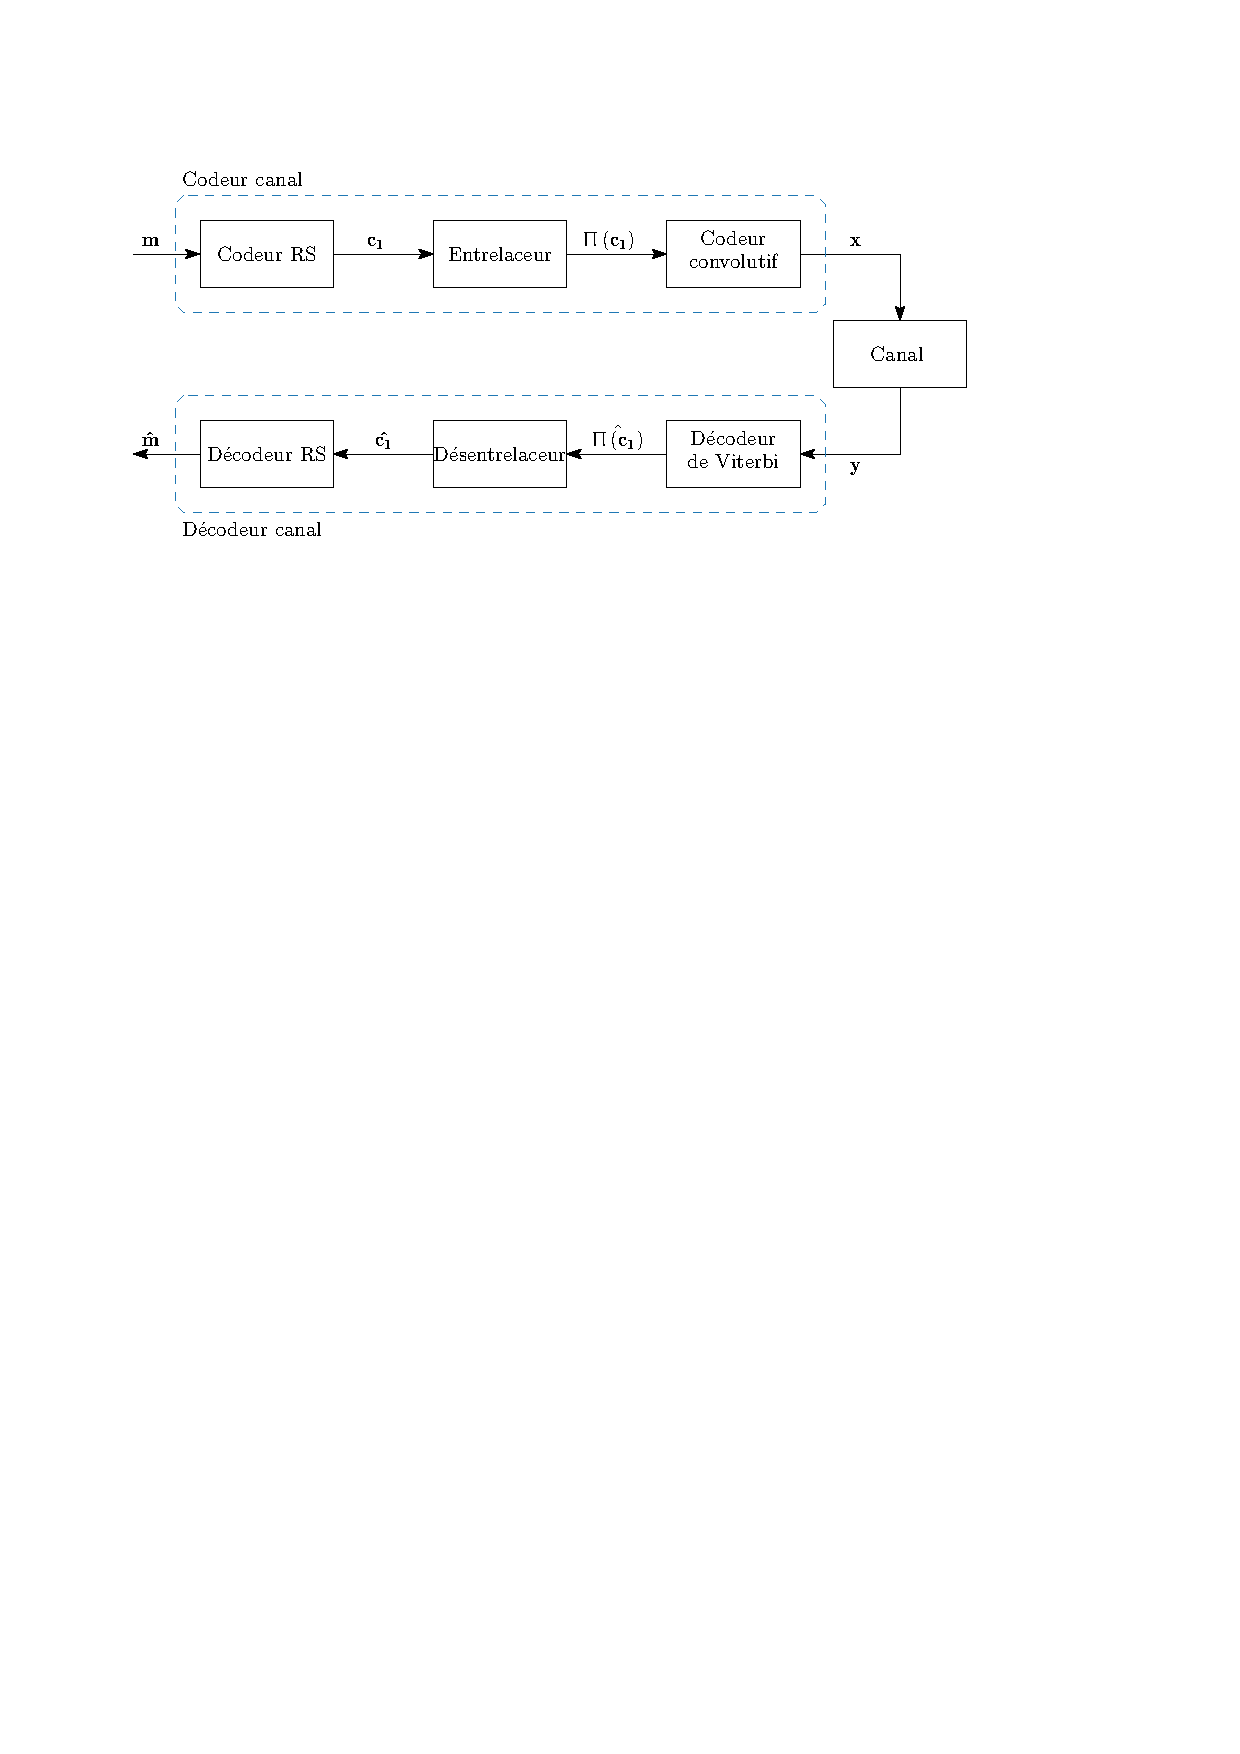
\includegraphics[width=12cm]{main/ch1_fig/nasa.pdf}
	\caption{\label{fig:nasa} Principe de concaténation série standardisé par la NASA}
\end{figure}

À la fin des années 80, Hagenauer et Hoeher proposent la concaténation série de codeurs convolutifs \cite{hagenauerConcatenated}.
À partir d'un décodeur SOVA \cite{BerrouHardwareSOVA}, Berrou s’attelle à expérimenter le décodage de cette 
concaténation série. Il décide alors de réinjecter la sortie du second décodeur (le décodeur extérieur) dans le premier
(le décodeur intérieur). Pour ce faire, il est nécessaire de reconstruire $\hat{c_1}$ après décodage par le décodeur extérieur.
C'est alors que Berrou remarque que le BER de ces symboles reconstruits est inférieur à celui du mot décodé $\hat{c}$. 
Cette constatation n'avait alors jamais été décrite dans la littérature. Il restait alors à remplacer les codeurs constitutifs 
par des versions systématiques. Ainsi, la sortie du second décodeur pouvait être réinjectée à l'entrée du premier.
Mais les codes convolutifs systématiques ont des propriétés moins intéressantes que les codes convolutifs non-systématiques, 
à moins qu'il s’agisse d'un code convolutif récursif systématique, dit RSC. L'étude des codes RSC fut donnée à Punya Thitimajshima
dans le cadre de sa thèse \cite{rscTheseTelecom}.

L'idée de la \emph{concaténation parallèle} est concomitante à la démarche d'implémentation matérielle de la 
concaténation série des codes RSC. En effet, une architecture matérielle de schéma concaténé en série -- de part les 
différents rendements des codes constituants -- nécessite différentes horloges. La concaténation parallèle simplifie ce
problème puisque les deux codeurs constitutifs et les deux décodeurs constitutifs fonctionnent avec la même horloge. De plus,
cette nouvelle structure permet aussi, à rendement égal, d'obtenir plus de symboles redondants pour un des deux codeurs 
élémentaires 
%qu'avec une concaténation classique (série)
. Par exemple, pour obtenir un code concaténé de rendement 1/3, 
dans le cas d'une concaténation parallèle, les deux codeurs auront un rendement 1/2. En revanche, pour une
concaténation série, l'un aura un rendement 1/2 et l'autre un rendement 2/3. En effet, si $R_p$ est le rendement 
global obtenu pour la concaténation parallèle de 2 codeurs de rendement $R_1$ et $R_2$ et $R_s$ celui obtenu pour une 
concaténation série, ils ont respectivement pour expression : 
\[R_p = \frac{R_1 \times R_2}{R_1 + R_2 - R_1 \times R_2} \ \ \ \text{et} \ \ \ R_s = R_1 \times R_2\]
Finalement, cette plus grande diversité, provenant d'un plus grand nombre d'information redondante par information 
systématique, permet d'obtenir un seuil de convergence qui se produit à plus faible SNR. Ce 
seuil de convergence permet au schéma concaténé en parallèle de s'approcher à seulement 0.7 dB de la limite de Shannon 
\cite{berrouTC}. Néanmoins, les schémas concaténés en série permettent d'obtenir des distances minimales plus 
importantes impliquant de meilleures performances asymptotiques \cite{declercq2014channel}. Dans la littérature, afin de distinguer
ces deux types de turbo codes, les notations PCCC pour codes convolutifs concaténés en parallèle et SCCC pour codes
concaténés en série sont utilisés.

Les éléments constitutifs d'un turbo code concaténé en parallèle, comme présenté en Figure \ref{fig:turboEnc}, sont 
maintenant détaillés. Dans un premier temps, les codeurs RSC, puis l'entrelaceur et enfin le principe de poinçonnage sont 
traités dans la suite de cette section.

\begin{figure}[!h]
	\centering
	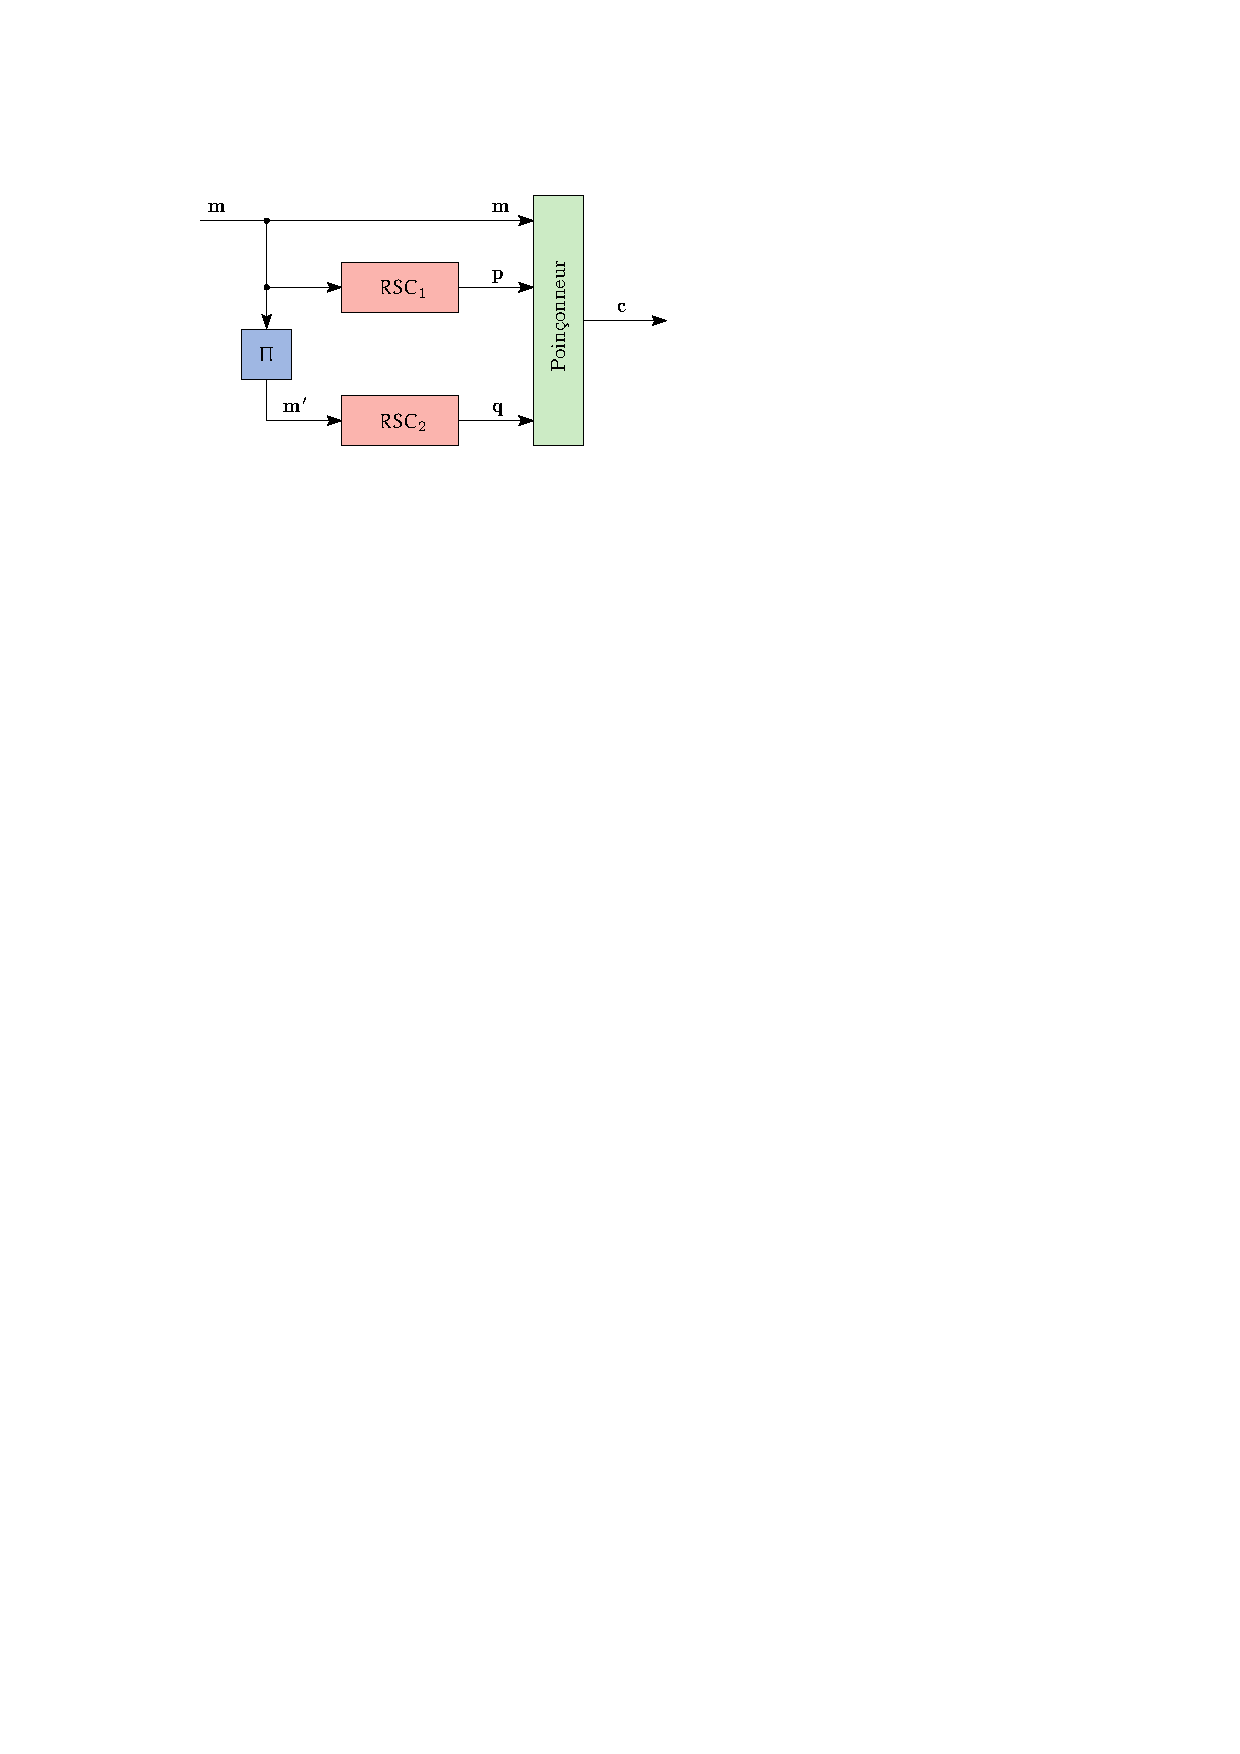
\includegraphics[width=8cm]{main/ch1_fig/turboEnc.pdf}
	\caption{\label{fig:turboEnc} Schéma générique d'un codeur de turbo code}
\end{figure}


\subsubsection{Codeur convolutif récursif}
Depuis les travaux de Forney, la concaténation de codes repose sur le codage de la séquence d'information par de multiples codeurs 
constitutifs à faible complexité calculatoire. Dans le cadre des turbo codes convolutifs, il s'agit de codes RSC à 4, 8 ou 16 états.
Augmenter le nombre d'états du codeur revient à accroître la distance minimale du code mais implique aussi une augmentation 
de la complexité calculatoire du décodeur. Les meilleurs codes RSC de rendement 1/2 adaptés aux turbo codes ont été identifiés 
et leurs distances minimales ont été calculées dans \cite{RSCdist}. Ces résultats sont reportés dans le tableau \ref{tab:bestRSC}. 
Les distances minimales sont relativement faibles. Dès lors, les performances asymptotiques des turbo codes résultent de l'étape 
d'entrelacement. 

\begin{table}[h]
	\centering
	\renewcommand{\arraystretch}{1.4}
	\begin{tabular}{rlll}
		\toprule
		\textbf{Nombre d'états}       & $\mathbf{4}$                           & $\mathbf{8}$                               & $\mathbf{16}$                                  \\ 
		\cmidrule(l){2-2} \cmidrule(l){3-3} \cmidrule(l){4-4}
		$\mathbf{G(D)}$                & $\left[1,\frac{1+D+D^2}{1+D^2}\right]$ & $\left[1,\frac{1+D+D^3}{1+D^2+D^3}\right]$ & $\left[1,\frac{1+D^3+D^4}{1+D+D^2+D^4}\right]$ \\
		$\mathbf{d_{min}/A_{d_{min}}}$ & 5/2                                    & 6/1                                        & 7/3                                            \\ \bottomrule
	\end{tabular}
	\caption{Codeurs RSC usuellement utilisés pour des turbo codes à 4, 8 et 16 états avec leur distance minimale et la multiplicité associée}
	\label{tab:bestRSC}
\end{table}

\subsubsection{Entrelacement}\label{sec:entrelacement}
Le premier but de l'entrelacement est de lutter contre les paquets d'erreurs. Ainsi lors de l'étape d'entrelacement, la 
séquence d'information dans \emph{l'ordre naturel} est mélangée par une fonction de permutation. Cette séquence est ensuite 
présentée dans \emph{l'ordre entrelacé} au second codeur RSC. Les propriétés de dispersion d'une permutation peuvent être mesurées en trouvant le minimum de la somme de la distance spatiale entre deux indices dans l'ordre naturel et dans l'ordre entrelacé. Cet écart (spread en anglais) est défini dans \cite{crozier2000new} par : 
\[S_{min} = \min\limits_{i_1, i_2, i_1 \ne i_2} \left( |i_1 - i_2| + |\Pi(i_1) - \Pi(i_2)| \right), \forall (i_1, i_2) \in \llbracket 0, K-1 \rrbracket ^2, \]
avec K la taille de l'entrelaceur et $\Pi$ la fonction d'entrelacement. 
Il a été démontré \cite{crozier2000new} que l'écart minimum a pour borne supérieure $\lfloor{\sqrt{2K}}\rfloor $.

Finalement, une bonne permutation doit permettre d'obtenir un écart suffisant afin de minimiser la corrélation entre les deux dimensions. Aussi, elle doit permettre d'atteindre de grandes distances minimales pour assurer de bonnes performances asymptotiques tout en pouvant être facilement implémentée. Ainsi, de part son rôle clef, la conception  d'entrelaceurs efficaces a été particulièrement étudiée dans la littérature. Dans la suite, quatre types d'entrelaceurs sont détaillés :
\begin{itemize}
	\item L'\emph{entrelaceur uniforme} n'est pas un cas pratique d'entrelaceur. Il ne peut être utilisé pour un standard de communication. Il a été défini par Benedetto en 1995 dans \cite{benedettoAverage} afin d'estimer les performances moyennes des schémas concaténés. Le principe de l'entrelaceur uniforme est de permuter un mot d'information de taille $K$ et de poids $w$ en un autre mot de poids $w$ parmi toutes les combinaisons possibles $\dbinom{K}{w}$, ce avec une probabilité équirépartie. Pour tout mot d'information, la permutation est choisie aléatoirement. Ainsi, cet entrelaceur permet d'extraire les paramètres des codes constituants d'un schéma concaténé sans avoir à tenir compte de la permutation.
	\item La permutation \emph{dithered relatively prime (DRP)} a été pensée par Crozier \cite{crozierDRP}. Elle est basée sur deux opérations de désordres (dither) séparées par une permutation régulière basée sur un entier premier relatif. Les entrelaceurs DRP ont l'avantage de pouvoir être facilement calculés en temps réel tout en permettant d'atteindre de bonnes performances asymptotiques. Néanmoins, ils n'ont jamais été standardisés.
	\item La \emph{permutation presque régulière (ARP)} a été développée par Berrou et son équipe en 2004 \cite{BerrouARP}. Elle est de la forme $j=\Pi(i)=Pi+Q(i)~~\text{mod}~~K$, avec $P$ premier et $K$ et $Q(j)$ entiers. Le nombre de valeurs différentes pour $Q(j)$ est souvent fixé à 4. Ce type de permutation a été choisi dans le cadre des standards de télédiffusion DVB-RCS \cite{dvbrcs},  DVB-RCS2 \cite{dvbrcs2} et  DVB-RCT \cite{dvbrct}. Cet entrelaceur possède l’avantage de présenter un parallélisme égal au cardinal de $Q(i)$. Cette propriété est intéressante pour l'implémentation de décodeurs rapides. 
	\item Enfin les entrelaceurs basés sur des \emph{permutations polynomiales quadratiques (QPP)} \cite{sunQPP} sont utilisés dans le standard de téléphonie de quatrième génération \cite{lte}. Cet entrelaceur est souvent de la forme $j=\pi(i)=f_1 i^2 + f_2 i~~\text{mod}~~K$, avec $f_1$ et $f_2$ entiers. La conception de ces entrelaceurs se réduit donc à trouver des coefficients polynomiaux. Ils permettent d'obtenir des distances minimales importantes \cite{rosnesQPP}. Ce type de permutation possède l'avantage de pouvoir être construite en respectant des propriétés de non contention. Ceci confère des possibilités de hauts degrés de parallélisme pour la conception du décodeur associé \cite{takeshitaQPP}.  
\end{itemize}
Récemment, il a été montré que ces 3 trois types d'entrelaceurs sont équivalents \cite{EquivalenceInt}. En effet, les permutations DRP et QPP peuvent s'écrire sous la forme d'une ARP. Ainsi, le formalisme lié à l'entrelaceur ARP devrait être le seul conservé à l'avenir.

Il est à noter que selon le type de fermeture du treillis ({\it cf.} \ref{par:term}), la terminaison peut être ou non incluse dans la séquence entrelacée. Ceci peut modifier les performances asymptotiques en impactant la distance minimale du code.

\subsubsection{Poinçonnage}
L'intérêt du poinçonnage est de supprimer certains bits de la séquence codée afin d'augmenter le rendement. Par exemple, le codeur présenté en Figure \ref{fig:turboEnc} possède un rendement nominal de $\frac{1}{3}$. Si nous supprimons à tour de rôle une des deux informations redondantes, le rendement du code devient $\frac{1}{2}$. Usuellement, seuls des symboles de redondance sont supprimés. Le poinçonnage est souvent représenté sous forme matricielle comme dans les équations \ref{eq:mat}. La première ligne correspond au poinçonnage de l'information redondante produite dans l'ordre naturel et la seconde ligne, celle produite dans l'ordre entrelacé. Un 1 signifie que le symbole est gardé, un 0 qu'il est poinçonné. Ainsi, à partir d'un turbo code de rendement natif de $\frac{1}{3}$, les matrices de poinçonnage \ref{eq:mat1a} à \ref{eq:mat1c} élèvent son rendement à respectivement  $\frac{2}{5}$, $\frac{1}{2}$ et $\frac{2}{3}$. Cette construction aisée de codes à rendements plus élevés est un atout indéniable vis-à-vis des codes en blocs.

\begin{subequations}\label{eq:mat}
	\begin{minipage}{0.25\textwidth}
		\begin{align}
			\label{eq:mat1a}
			\begin{bmatrix}
			1 & 1 \\
			1 & 0 
			\end{bmatrix}
		\end{align}
	\end{minipage}
	\begin{minipage}{0.25\textwidth}
		\begin{align}
			\label{eq:mat1b}
			\begin{bmatrix}
			1 & 0 \\
			0 & 1 
			\end{bmatrix}
		\end{align}
	\end{minipage}
	\begin{minipage}{0.35\textwidth}
		\begin{align}
			\label{eq:mat1c}
			\begin{bmatrix}
			1 & 0 & 0 & 0 \\
			0 & 0 & 1 & 0 
			\end{bmatrix}
		\end{align}
	\end{minipage}
\end{subequations}

\subsection{Décodage itératif}
Comme exprimé précédemment, l'innovation majeure des turbo codes est d'obtenir des performances en terme de correction d'erreurs proche de la limite de Shannon tout en proposant un principe de décodage relativement simple. De par la présence de la phase d'entrelacement, un décodage MAP n'est pas possible. En effet, cela impliquerait des calculs sur un treillis composé d'un trop grand nombre d'états. Ainsi en même temps que Berrou \textit{et al.} proposent la construction des turbo codes, ils introduisent une méthode de décodage non optimale mais à faible complexité \cite{berrouTC}. Cette technique est basée sur un processus itératif. D'abord, chaque code RSC est traité par un décodeur associé. Mais, comme le code est systématique et que chaque sous-code provient du même mot d'information (présenté dans un ordre différent), les informations produites par les deux décodeurs peuvent être combinées. Ainsi, l'information délivrée par l'un des décodeurs est utilisée par le second. Le décodage itératif permet donc d'augmenter la fiabilité de la décision aux cours des itérations. L'information échangée par les décodeurs est appelée \emph{information extrinsèque}. Un schéma générique du décodeur itératif correspondant au codeur générique de la Figure \ref{fig:turboEnc} est présenté en Figure \ref{fig:turboDec}. Le principe du décodage itératif est désormais introduit.

\begin{figure}[!h]
	\centering
	\includegraphics[width=10cm]{main/ch1_fig/TurboDec.pdf}
	\caption{\label{fig:turboDec} Structure d'un décodeur de turbo code}
\end{figure}

%
	
% \subsection{Les turbo codes standardisés}
	
% % % \newpage
% % % Here you	 can see a citation: \cite{atc13}.\\
% % % Here you can see a glossary use \gls{lvm}.

\subsubsection{Décodage SISO : l'algorithme BCJR}\label{sec:BCJR}
Considérons un turbo code binaire sans poinçonnage composé de deux codeurs RSC de rendement $1/2$. La séquence d'information binaire de taille K $\mathbf{m} = (m_1, m_2, ..., m_K)$ est appliquée au premier codeur RSC. Sa sortie est notée par $\mathbf{c^p} = (c^p_1, c^p_2, ..., c^p_K)$. La séquence d'information est aussi entrelacée et devient $\mathbf{m'} = (m'_1, m'_2, ..., m'_K)$. Cette dernière est ensuite codée par le second RSC afin d'obtenir $\mathbf{c'^p} = (c'^p_1, c'^p_2, ..., c'^p_K)$. La sortie du turbo codeur correspond alors à la concaténation de ces trois séquences $(\mathbf{m}, \mathbf{c^p}, \mathbf{c'^p})$. Une modulation numérique de type BPSK est employée afin de transmettre cette séquence sur un canal BI-AWGN. La sortie du démodulateur est notée par $(\mathbf{y^s},\mathbf{y^p},\mathbf{y'^p})$. Le premier décodeur SISO va alors travailler sur le couple $(\mathbf{y^s},\mathbf{y^p})$ et le second décodeur SISO sur le  couple $(\mathbf{y'^s},\mathbf{y'^p})$ tel que $y'^s = \Pi(y^s)$.

Deux principaux algorithmes peuvent être utilisés dans les décodeurs SISO. La condition nécessaire dans un contexte itératif est qu'ils fournissent des sorties pondérées. Ainsi, il peut s'agir de l'algorithme SOVA ou de l'algorithme BCJR modifié par Berrou \cite{berrouTC} afin de fournir des probabilités \textit{a posteriori} pour chaque symbole d'information. Ce dernier, puisqu'il utilise la règle de décision MAP, est aussi appelé  algorithme MAP. Néanmoins, comme cette version modifiée fournit des probabilités \textit{a posteriori}, la notation APP rencontrée dans la littérature est plus précise.

Il a été montré que l'algorithme SOVA possède une complexité calculatoire au moins deux fois plus faible que celle de l'algorithme APP \cite{robertson1995comparison}. Néanmoins, cette faible complexité calculatoire s'accompagne d'une dégradation des performances de décodage. C'est pourquoi, en pratique, l'algorithme APP est retenu lors de l'implémentation du décodeur SISO. Les calculs menés par l'un des décodeurs doivent être explicités. Cependant, afin de faciliter la lecture de cette section, les calculs intermédiaires sont déportés en Annexe \ref{append:app}.

Le principe du décodage à maximum \textit{a posteriori} symbole par symbole est de calculer pour tout $k\in \llbracket1;K\rrbracket$ : 
\begin{equation}
	\label{eq:maprule}
	\hat{m_k} = \argmax\limits_{u_k\in\{0,1\}} P(u_k| \mathbf{y}).	
\end{equation}

Cependant, si nous prenons en compte la représentation sous forme de treillis du codeur RSC, ce calcul est strictement équivalent à celui des probabilités de transitions formulé par : 
\[\hat{m_k} = \argmax_{i\in\{0,1\}} \sum\limits_{(s,s')\in\Gamma_{k,i}}P(s_{k-1}=s, s_{k}=s',\mathbf{y}),\]
où $\Gamma_{k,i}$ représente l'ensemble des chemins de la ${k^{ième}}$ section de treillis pour lesquels $u_k=i$. 

En exploitant les propriétés du treillis et la relation de Bayes, la probabilité jointe peut s'écrire sous la forme d'un produit de trois termes. Tout d'abord, $\mathbf{y}$ peut être décomposé en trois sous séquences : le passé exprimé par $\mathbf{y_{<k}}$, le présent $\mathbf{y_k}$ et le futur $\mathbf{y_{>k}}$. Ainsi $\mathbf{y} = (\mathbf{y_{<k}}, \mathbf{y_k}, \mathbf{y_{>k}}).$ La probabilité jointe a alors pour expression : 
\begin{align*}
	P(s_{k-1}=s, s_{k}=s',\mathbf{y}) & = P(s_{k-1}=s, s_{k}=s',\mathbf{y_{<k}},\mathbf{y_{k}},\mathbf{y_{>k}})                                                                                                                              \\
	                                  & = \underbrace{P(\mathbf{y_{>k}}|s_{k}=s')}_{\beta_k(s')}\times \underbrace{P(s_{k}=s',\mathbf{y_{k}}|s_{k-1}=s)}_{\gamma_k(s,s')}\times \underbrace{P(s_{k-1}=s,\mathbf{y_{<k}}).}_{\alpha_{k-1}(s)} 
\end{align*}
Chaque calcul de probabilité jointe est donc ramené au produit de trois termes :
\begin{itemize}
	\item la probabilité d'état aller : $\alpha_{k-1}(s)$, représentant la probabilité qu'à l'instant k-1 l'état courant dans le treillis soit s et que la séquence reçue jusqu'alors soit $\mathbf{y_{<k}}$,
	\item la probabilité d'état retour : $\beta_k(s')$, représentant la probabilité qu'à l'instant k la future séquence soit $\mathbf{y_{>k}}$ sachant que l'état courant est $s'$,
	\item la probabilité de transition : $\gamma_k(s,s')$ représente la probabilité qu'à l'instant k l'état courant soit $s'$ et que le symbole reçu soit $\mathbf{y_k}$ sachant que l'état précédent est $s$.
\end{itemize}
\paragraph*{Calcul des probabilités d'état}
De part leur définition, les probabilités d'état peuvent être exprimées récursivement. Ainsi, 
\begin{equation}	\begin{split}
	\alpha_k(s)=\sum\limits_{s'}\alpha_{k-1}(s')\gamma_k(s,s')
	\end{split}\qquad\text{et}\qquad
	\begin{split}
		\beta_{k-1}(s)=\sum\limits_{s'}\beta_{k}(s')\gamma_k(s,s').
	\end{split} 
\end{equation}
En supposant que le treillis commence et termine dans l'état $s_0$, les conditions initiales pour ces deux probabilités sont : 
\[
	\begin{split}
		\alpha_0(s)=\begin{cases}
		1 \text{~~si~~} s = s_0 \\
		0 \text{~~sinon~~}
		\end{cases}
	\end{split}\qquad\qquad\text{et}\qquad\qquad
	\begin{split}
		\beta_K(s)=\begin{cases}
		1 \text{~~si~~} s = s_0 \\
		0 \text{~~sinon~~}
		\end{cases}
	\end{split}
\]
			
\paragraph*{Calcul des probabilités de transition} Tout d'abord, il est à noter que si la transition dans une tranche de treillis entre l'état $s$ et l'état $s'$ n'existe pas, alors $\gamma_k(s,s')=0.$
Ensuite, en partant de la définition de $\gamma_k$ et en utilisant la relation de Bayes, nous obtenons : 
\[\gamma_k(s,s') = P(m_k)P(\mathbf{y_k}|{c_k}).\]
Puisque nous considérons que le message produit par la source est équiprobable, nous avons $P(m_k) = 1/2$. Ensuite, en reprenant l'équation \ref{eq:p(y|x)} établissant la probabilité conditionnelle liant la sortie et l'entrée d'un canal AWGN, nous obtenons : 
\begin{equation*}
	\gamma_k(s,s') = P(m_k)\frac{1}{(2\pi\sigma^2)} \exp \left(-\frac{\|\mathbf{y}_k-\mathbf{c}_k\|^2}{2 \sigma^2}\right),
\end{equation*}
avec $\mathbf{y}_k = (y^s_k, y^p_k)$ et $\mathbf{c}_k = (c^s_k, c^p_k)$. Finalement, en développant la norme et en supprimant les termes ne dépendant pas de $m_k$ qui se simplifieront dans le calcul suivant, nous obtenons : 
\begin{equation}	\label{eq:llr}
	\gamma_k(s,s') = P(m_k) \exp \left(\frac{y^s_k c^s_k + y^p_k c^p_k}{\sigma^2}\right),
\end{equation}

\paragraph*{Calcul des probabilités \textit{a posteriori}} L'équation \ref{eq:maprule} permet d'obtenir la décision dure $\hat{m_k}$. Cependant, dans le cadre d'un décodage itératif, il est nécessaire d'avoir une valeur pondérée -- représentant la fiabilité de cette décision -- exprimée sous forme d'un logarithme de rapport de vraisemblance (LLR) : 
\begin{align}
	L(m_k) & = \ln\frac{P(m_k=1|\mathbf{y})}{P(m_k=0|\mathbf{y})}                                                                                                                           \\
	       & = \ln\frac{\sum\limits_{(s,s')\in\Gamma_{k,1}} \alpha_{k-1}(s) \gamma_k(s,s') \beta_k(s)}{\sum\limits_{(s,s')\in\Gamma_{k,0}}\alpha_{k-1}(s) \gamma_k(s,s') \beta_k(s)} \notag 
\end{align}
Toujours dans le cas d'un codeur RSC de rendement 1/2, d'une modulation BPSK (prenant les 2 valeurs possibles $\pm1$) et d'un canal BI-AWGN, le LLR peut être décomposé en trois éléments :
\begin{align}
	\label{eq:app}
	L(m_k) & =  \ln\frac{\sum\limits_{(s,s')\in\Gamma_{k,1}} \alpha_{k-1}(s) \cdot P(m_k) \exp \frac{y_k^sc_k^s+y_k^pc_k^p}{\sigma^2} \cdot \beta_k(s)}{\sum\limits_{(s,s')\in\Gamma_{k,0}} \alpha_{k-1}(s)\cdot  P(m_k) \exp \frac{y_k^sc_k^s+y_k^pc_k^p}{\sigma^2} \cdot \beta_k(s)}        \notag                             \\
	       & =  \frac{2}{\sigma^2}y_k^s + \ln \frac{P(m_k=1)}{P(m_k=0)} + \ln\frac{\sum\limits_{(s,s')\in\Gamma_{k,1}} \alpha_{k-1}(s) \cdot P(m_k) \exp \frac{y_k^pc_k^p}{\sigma^2} \cdot \beta_k(s)}{\sum\limits_{(s,s')\in\Gamma_{k,0}} \alpha_{k-1}(s)\cdot  P(m_k) \exp \frac{y_k^pc_k^p}{\sigma^2} \cdot \beta_k(s)}\notag \\
	       & = L_cy_k^s\qquad~ + L^a(m_k)\qquad~ + L^e(m_k)                                                                                                                                                                                                                                                                      
\end{align}
Le premier terme correspond à l'effet du canal sur les bits systématiques. Le second est l'information \textit{a priori}. Enfin le dernier terme est l'information extrinsèque qui ne dépend ni des probabilités a priori, ni de l'information systématique.

Ainsi, lors du décodage itératif d'un turbo code (cf. Figure \ref{fig:turboDec}), le décodeur $SISO_1$ reçoit le couple $(\mathbf{y^s},\mathbf{y^p})$. À partir de l'équation \ref{eq:app}, les LLR \textit{a posteriori} sont calculés en considérant les LLR \textit{a priori} nuls. En effet, les bits d'information sont équiprobables. Ensuite, afin d'en extraire les informations extrinsèques (notées $\mathbf{L^e_{12}}$), les informations du canal correspondant aux bits systématiques sont soustraites. L'information extrinsèque est alors traitée par l'entrelaceur $\Pi$. Elles sont alors utilisées en tant qu'information \textit{a priori} par le décodeur $SISO_2$ conjointement avec $(\mathbf{y'^s},\mathbf{y'^p},)$ pour fournir les informations extrinsèques (notées $\mathbf{L^e_{21}}$). Ces dernières sont permutées selon $\Pi^{-1}$ afin que le $SISO_1$ les utilise lors de l'itération suivante dans le domaine naturel en tant qu'information \emph{a priori}. 

Ce processus est répété jusqu'à ce que ce qu'un nombre fixé d'itérations soit atteint ou jusqu'à ce qu'un critère d’arrêt soit vérifié.

Comme présenté précédemment, l'algorithme APP a pour principal inconvénient sa complexité calculatoire. Cette dernière provient du nombre conséquent de multiplications et de calculs d'exponentielles. Afin de réduire cette complexité calculatoire plusieurs simplifications ont été proposées.

\subsubsection{Simplifications de l'algorithme APP}
La simplification de l'algorithme APP passe par la transposition dans le domaine logarithmique des différentes probabilités calculées. Cette version se nomme log-APP. Les détails des calculs sont présentés en Annexe \ref{append:subAPP}.

Les probabilités précédentes sont alors remplacées par les métriques suivantes : 
\begin{itemize}
	\item La métrique d'état aller : $~\tilde{\alpha}_k(s) = \ln \alpha_k(s)$,
	\item La métrique d'état retour : $\tilde{\beta}_k(s) = \ln \beta_k(s)$,
	\item La métrique de branche : $\tilde{\gamma}_k(s, s') = \ln \gamma_k(s, s')$.\\
\end{itemize}

En introduisant l'opérateur  $\maxstar$ défini par $\maxstar(x,y) = \ln(\e^x+ \e^y)$, il vient naturellement :
\begin{align*}
	% ~\tilde{\alpha}_k(s)    & = \ln \sum\limits_{s'} \exp\left(\tilde{\alpha}_{k-1}(s') + \tilde{\gamma}_k(s', s)\right) \quad\text{et} \\
	% ~\tilde{\beta}_{k-1}(s) & = \ln \sum\limits_{s'} \exp\left(\tilde{\beta}_{k}(s') + \tilde{\gamma}_k(s', s)\right) .         
	~\tilde{\alpha}_k(s)    & = \maxstar\limits_{s'}\left(\tilde{\alpha}_{k-1}(s') + \tilde{\gamma}_k(s', s)\right) 
	\quad\text{et} \\
	~\tilde{\beta}_{k-1}(s) & = \maxstar\limits_{s'} \left(\tilde{\beta}_{k}(s') + \tilde{\gamma}_k(s', s)\right)   
\end{align*}
Les conditions initiales sont dorénavant : 
\[
	\begin{split}
		\tilde{\alpha}_0(s)=\begin{cases}
		0 \qquad\text{si~~} s = s_0 \\
		-\infty \qquad\text{sinon}
		\end{cases}
	\end{split}\qquad\text{et}\qquad
	\begin{split}
		\tilde{\beta}_K(s)=\begin{cases}
		0 \qquad\text{si~~} s = s_0 \\
		-\infty \qquad\text{sinon}
		\end{cases}
	\end{split}
\]
Finalement les valeurs \textit{a posteriori} deviennent : 
\begin{align}
	L(m_k) 	= \maxstar\limits_{(s,s')\in\Gamma_{k,1}} & \left(\alpha_{k-1}(s) \gamma_k(s,s') \beta_k(s)\right) \notag \\&- \maxstar\limits_{(s,s')\in\Gamma_{k,0}}\left(\alpha_{k-1}(s) \gamma_k(s,s') \beta_k(s)\right).				
\end{align}
Cependant, en l'état, la complexité calculatoire demeure. C'est pourquoi, un travail complémentaire sur l'opérateur $\maxstar$ est nécessaire. Ainsi, il est aisément démontrable (cf \ref{append:maxstar}) que : 
\[\maxstar(x,y)=\max(x,y) +\ln\left(1+\e^{-|x-y|}\right) \]
Les différentes simplifications de l'algorithme log-APP vont alors consister en des approximations plus ou moins fines du terme logarithmique, noté dans la suite $f_c(x,y)$.

La première approximation est nommée constant-log-APP \cite{constantlog1}. Si la différence $|x-y|$ est inférieure à un seuil, alors une constante de correction est ajoutée à la valeur du maximum : 
\begin{equation}
	\maxstar(x,y)=\max(x,y) + \begin{cases} 0 \qquad\text{si~~} |x-y| > T \\
	C \qquad\text{si~~} |x-y| \leq T. \end{cases}
\end{equation}
Dans \cite{constantlog2}, les valeurs présentées pour $T$ et $C$ valent respectivement $1,5$ et $0,5$.

Dans le cadre du linear-log-APP, le terme logarithmique est approximé par une fonction affine \cite{linearlog} : 
\begin{equation}
	\maxstar(x,y)=\max(x,y) + \begin{cases} 0 \qquad\text{si~~} |x-y| > T \\
	a(|y-x|-T) \qquad\text{si~~} |x-y| \leq T, \end{cases}
\end{equation}
avec $a=0.24904$ et $T=2.5068$.

Finalement, la dernière approximation consiste à ne pas ajouter de terme de correction. Ainsi, l'opérateur $\maxstar$ est remplacé uniquement par l'opérateur $\max$. Cette approximation, appelée max-log-APP (ML-APP) est celle à plus faible complexité calculatoire. Cependant les performances de décodage se situent alors à environ $0,5$ dB de celles de l'algorithme log-APP.

Ces trois différentes approximations sont récapitulées dans la Figure \ref{fig:logapprox}. Au niveau des performances de décodage, plus l'approximation a une complexité calculatoire élevée, plus elle se rapproche de la fonction originelle et donc des performances optimales. Des comparaisons des impacts de ces approximations sont présentées dans \cite{robertson1995comparison} et \cite{logapprox}.
\begin{figure}[!h]
	\centering
	%!TEX root = ../../my_thesis.tex
\begin{tikzpicture}
	\begin{axis}[footnotesize, width=0.8\linewidth, height=0.55\linewidth,    
			xmin=0, xmax=4, xtick={0, 0.5,...,4},
			ymin=-0.1,  ymax=0.8, ytick={-0.1, 0,...,0.8},
			xlabel=$|x-y|$, ylabel=Fonction de correction ($f_c(x-y)$),  grid=both, grid style={gray!30},
			tick align=outside, tickpos=left
			]
		%legend pos=outer north]
 		\addplot[Paired-1,domain=0:4, samples=400,semithick]{ln(1+exp(-x))};
 		\addplot[Paired-3,domain=0:2.5, samples=200,semithick]{-0.24905*(x-2.5068)};
 		\addplot[Paired-5,domain=0:1.5, samples=50,semithick]{0.5};
 		\addplot[Paired-7,domain=0:4, samples=50,semithick]{0};
 		\draw[dotted, Paired-5,semithick] (axis cs:1.5,0.5) -- (axis cs:1.5,0);

 		\addplot[Paired-3,domain=2.5:4.0, samples=50,semithick]{0.003};
		\addplot[Paired-5,domain=1.5:4.0, samples=50,semithick]{0.001};

		\legend{log-APP, 			linear-log-APP,			constant-log-APP, 			max-log-APP}
		
	\end{axis}
\end{tikzpicture}  
	\caption{\label{fig:logapprox} Fonctions des correction des différentes approximations de l'algorithme log-APP} 
\end{figure}

Cependant, en 2000, il a été proposé d'utiliser un facteur d'échelle sur l'information extrinsèque avant qu'elle soit utilisée par le décodeur SISO suivant \cite{enhancedmlmap}. Cette méthode, appelée enhanced-max-log-APP (EML-APP), est inspirée de \cite{HagenHoerViter} dans le cadre de l'algorithme SOVA. En effet, il avait été remarqué que les valeurs des LLR calculés par les décodeurs SISO étaient sur-évaluées.
Ce facteur d'échelle (SF) peut être constant au cours du processus itératif. Dans ce cas, la valeur de $0,75$ est souvent choisie. En effet, elle peut être facilement réalisée en sommant un décalage vers la gauche de 2 et un décalage vers la gauche de 1. Autrement, la remise à l'échelle peut être adaptative. Le facteur évolue alors de $0,5$ pour la première itération jusqu'à $1.0$ pour la dernière. En moyenne, grâce à l'utilisation de ce facteur, les performances de décodage avec l'EML-APP ne se situent plus qu'à $0.1$ dB de celles du log-APP.
Dans \cite{scaling}, l'influence de la valeur du facteur d'échelle est étudiée afin de minimiser le BER et le FER.


\subsection{Les turbo codes double binaires}\label{sec:dbl}
En 1999, les turbo codes non binaires ont été introduits \cite{doublebin1}. À la différence des turbo codes binaires, les turbo codes double binaires traitent $2$ bits en parallèle. Il en découle que les codeurs RSC constituants sont eux mêmes double binaires. Pour ce faire, des extensions multi binaires ont été développées. Le codeur constitutif employé est alors de rendement nominal $m/(m+1)$ avec $m$ le nombre de donnés simultanément présentes à l'entrée du codeur \cite{doublebin3}. La figure \ref{fig:encMulti} présente un tel codeur sans faire apparaître la sortie pour des soucis de lisibilité. Il est toute fois à noter qu'utiliser $m > 2$ n'apporte qu'un intérêt limité pour des RSC de mémoire 3 ou 4 \cite{Balta2013}. En effet, trop peu de diversité dans l'interconnexion ne peut être obtenus dans de tels cas.
\begin{figure}[!h]
	\centering
	\includegraphics[width=10cm]{main/ch1_fig/encMulti.pdf}
	\caption{\label{fig:encMulti} Structure générique d'un codeur RSC $m$-binaire et de taille de contrainte $\nu +1$}
\end{figure}

Pour le cas double binaire, le rendement des codes constituants est donc $2/3$. Le rendement nominal du turbo code obtenu est donc $1/2$. Cependant, il est possible d'ajouter une seconde sortie  d'information redondantes, pour chaque code constituant, afin d'obtenir un turbo code de rendement $1/3$. 

Selon \cite{doublebinadvantages}, les avantages des turbo codes double binaires sont les suivants : 
\begin{itemize}
	%\item meilleure convergence,
	\item plus grande distance minimale,
	\item moindre poinçonnage : puisque le turbo code est de rendement nominal 1/2, moins de poinçonnage -- comparativement aux turbo codes binaires -- est nécessaire pour atteindre de forts rendements,
	\item latence réduite : puisque les données sont traitées par groupe de deux bien qu'il y ait plus de calculs par tranche de treillis à mener,
	\item robustesse du décodeur : la dégradation au niveau des performances entre l'algorithme MAP et ses versions simplifiées est moins importante que dans le cadre binaire.
\end{itemize}

Dans la littérature, l'entrée des codeurs constituants est dénoté par le couple $(A_k,B_k)$. Les sorties correspondantes sont notées $(Y_k,W_k)$. Si la trame a coder contient $K$ bits, alors $K/2$ symboles sont codés. Dans ce cas, nous avons $k \in \llbracket 0, K/2-1\rrbracket$.

L'emploi de codes double binaires permet un entrelacement des données sur deux niveaux. Le premier agit au niveau intra-symboles et le second au niveau inter-symboles. Ainsi, la première permutation consiste à permuter l'ordre du couple tous les deux symboles : si $k$ est pair, $(A_k,B_k)$ devient $(B_k,A_k)$. Pour le second niveau d'entrelacement, une permutation comme celles présenté en section \ref{sec:entrelacement} est appliquée.

Le décodage des turbo codes double binaires est basé sur une extension de l'algorithme log-APP. Cependant, au lieu de calculer un seul LLR par tranche de treillis, il faut, dans ce cas, en calculer trois. En effet, selon \ref{eq:llr}, chaque LLR correspond au rapport entre la probabilité qu'un 1 soit émis et la probabilité qu'un 0 soit émis. Dans le cadre double binaire, il s'agit de calculer le rapport entre la probabilité de chaque symbole possiblement émis et la probabilité qu'un symbole 0 soit émis. Ceci est exprimé par : 
\begin{equation*}
	L_{(a,b)}(A_k,B_k) = \ln\frac{P(A_k=a,B_k=b|\mathbf{y})}{P(A_k=0,B_k=0|\mathbf{y})},
\end{equation*}
avec (a,b) valant (0,1), (1,0) ou (1,1).

Il en suit que lors du processus itératif, trois valeurs extrinsèques sont échangées par tranche du treillis.
Finalement, les décisions binaires sont prises en testant le signe de : 
\begin{align*}
	L(A_k) & = \maxstar \left(L_{(1,0)}(A_k,B_k),L_{(1,1)}(A_k,B_k)\right) - \maxstar \left(L_{(0,1)}(A_k,B_k),0\right) \\
	L(B_k) & = \maxstar \left(L_{(0,1)}(A_k,B_k),L_{(1,1)}(A_k,B_k)\right) - \maxstar \left(L_{(1,0)}(A_k,B_k),0\right) 
\end{align*}
puisque, par définition, $L^e_{(0,0)}(A_k,B_k)=0$.

Pour conclure, les turbo codes double binaires, tout comme leurs antécédents binaires ont été standardisés. Les principales caractéristiques de ces codes sont présentées en section suivante.

\subsection{Les turbo codes standardisés}
Peu après la publication des premiers résultats confirmant les performances de décodage des turbo codes, plusieurs comités de standardisation se sont intéressé à cette nouvelle famille de code correcteur d'erreurs.

Ainsi, en 1999, le Comité Consultatif pour les Systèmes de Données Spatiales (CCSDS, qui regroupe différentes agences spatiales à travers le monde), propose dans leur livre de recommandations d'employer un turbo code à 16 états dans le cadre des communications avec l'espace lointain \cite{ccsdsBluebook}. 

Aujourd'hui, nous retrouvons des turbo codes essentiellement dans des contextes de télécommunication mobile et de diffusion vidéo numérique.

Depuis la fin des années 90, le 3GPP a adopté un turbo code à 8 états dans le cadre de la technologie de téléphonie mobile de troisième génération UMTS. En même temps, son concurrent, le 3GPP2, fait de même pour la norme CDMA2000, avec un turbo code très proche de celui de l'UMTS mais proposant plus de rendements. 
Enfin, dans le cadre de la technologie de téléphonie mobile de quatrième génération, les standards LTE et LTE-Advanced \cite{lte} adoptent les mêmes codes constituants mais un nouvel entrelacement basé sur des permutations QPP est retenu.

Le consortium européen DVB, dès 1994, s'est intéressé aux turbo codes pour le standard de diffusion vidéo numérique terrestre DVB-T. Cependant, ce n'est qu'en 2000 que les turbo codes sont standardisés dans ce contexte afin d'assurer la voie retour permettant l'ajout de services tels que des programmes TV interactifs ou l’accès à internet. Ainsi deux standards, le DVB-RCS \cite{dvbrcs} et le DVB-RCT \cite{dvbrct} spécifient respectivement la voie retour du standard DVB-S et la voie retour du standard DVB-T. Ces deux turbo codes standardisés sont des codes double binaires 8 états et leur entrelaceur est basé sur une permutation ARP. Depuis 2012, la seconde génération du standard DVB-RCS2 \cite{dvbrcs2} comprend un turbo code similaire mais à 16 états.

D'autres standards utilisent des turbo codes tels que le WiMAX \cite{wimax} pour des  communications numériques sans fil. Les turbo codes sont aussi présents dans les standards HomePlug AV et HomePlug AV2 \cite{hpav} spécifiant des communications par courant porteur en ligne. Ces trois turbo codes sont similaires à celui du DVB-RCS.

Dans la suite de ce manuscrit, les standards CCSDS, LTE, DVB-RCS et DVB-RCS2 seront utilisés comme cadre applicatif, car à eux 4 ils représentent une diversité conséquente quant aux turbo codes usités. Le tableau \ref{tab:std} récapitule les propriété de ces turbo codes. Les treillis associés aux codeurs RSC élémentaires des turbo codes de chacun de ces standard sont présentés en Figure \ref{fig:treillisstd}. Les performances de décodage de ces turbos codes sont présentées, de manière non exhaustive, en Figures \ref{fig:ferstdlte} à \ref{fig:ferstdDVB2}. Pour toutes ces simulations Monte Carlo, 100 trames erronées ont été obtenues par point de SNR. L'algorithme de décodage est l'EML-APP avec comme facteur d'échelle $0,75$ durant 8 itérations.

\begin{table}[h]
	\centering
	\caption{Les turbo codes standardisés utilisés durant la thèse}
	\label{tab:std}
	\begin{tabular}{@{}rllll@{}}
		\toprule
		& \multicolumn{2}{l}{Binaire} & \multicolumn{2}{l}{Double binaire} \\ 
		\cmidrule(l){2-3}\cmidrule(l){4-5}
		                        & \textbf{LTE}          & \textbf{CCSDS}          & \textbf{DVB-RCS}      & \textbf{DVB-RCS2}      \\
		\cmidrule(l){2-2}\cmidrule(l){3-5}%\cmidrule(l){3-3}\cmidrule(l){4-4}\cmidrule(l){5-5}
		Type de communication                  & Mobiles       &  \multicolumn{3}{c}{Satellitaires}                 \\
		\cmidrule(l){2-2}\cmidrule(l){3-3}\cmidrule(l){4-4}\cmidrule(l){5-5}
		Nombre d'états         & 8                     & 16                      & 8                     & 16                     \\
		\cmidrule(l){2-3}\cmidrule(l){4-5}
		Terminaison du treillis    &     \multicolumn{2}{c}{Retour à l'état 0}               &                \multicolumn{2}{c}{Circulaire}                    \\
		\cmidrule(l){2-2}\cmidrule(l){3-3}\cmidrule(l){4-4}\cmidrule(l){5-5}
		Tailles de trame (bits) & $40 \rightarrow 6144$ & $1784 \rightarrow 8920$ & $96 \rightarrow 1728$ & $128 \rightarrow 3008$ \\
		\cmidrule(l){2-2}\cmidrule(l){3-3}\cmidrule(l){4-4}\cmidrule(l){5-5}
		Rendements              & Rate-Matching         & $1/6 \rightarrow 1/2$   & $1/3 \rightarrow 6/7$ & $1/3 \rightarrow 7/8$  \\ \bottomrule
	\end{tabular}
\end{table}

\begin{figure}[h!]
	\begin{center}
		\subfloat[LTE]{
			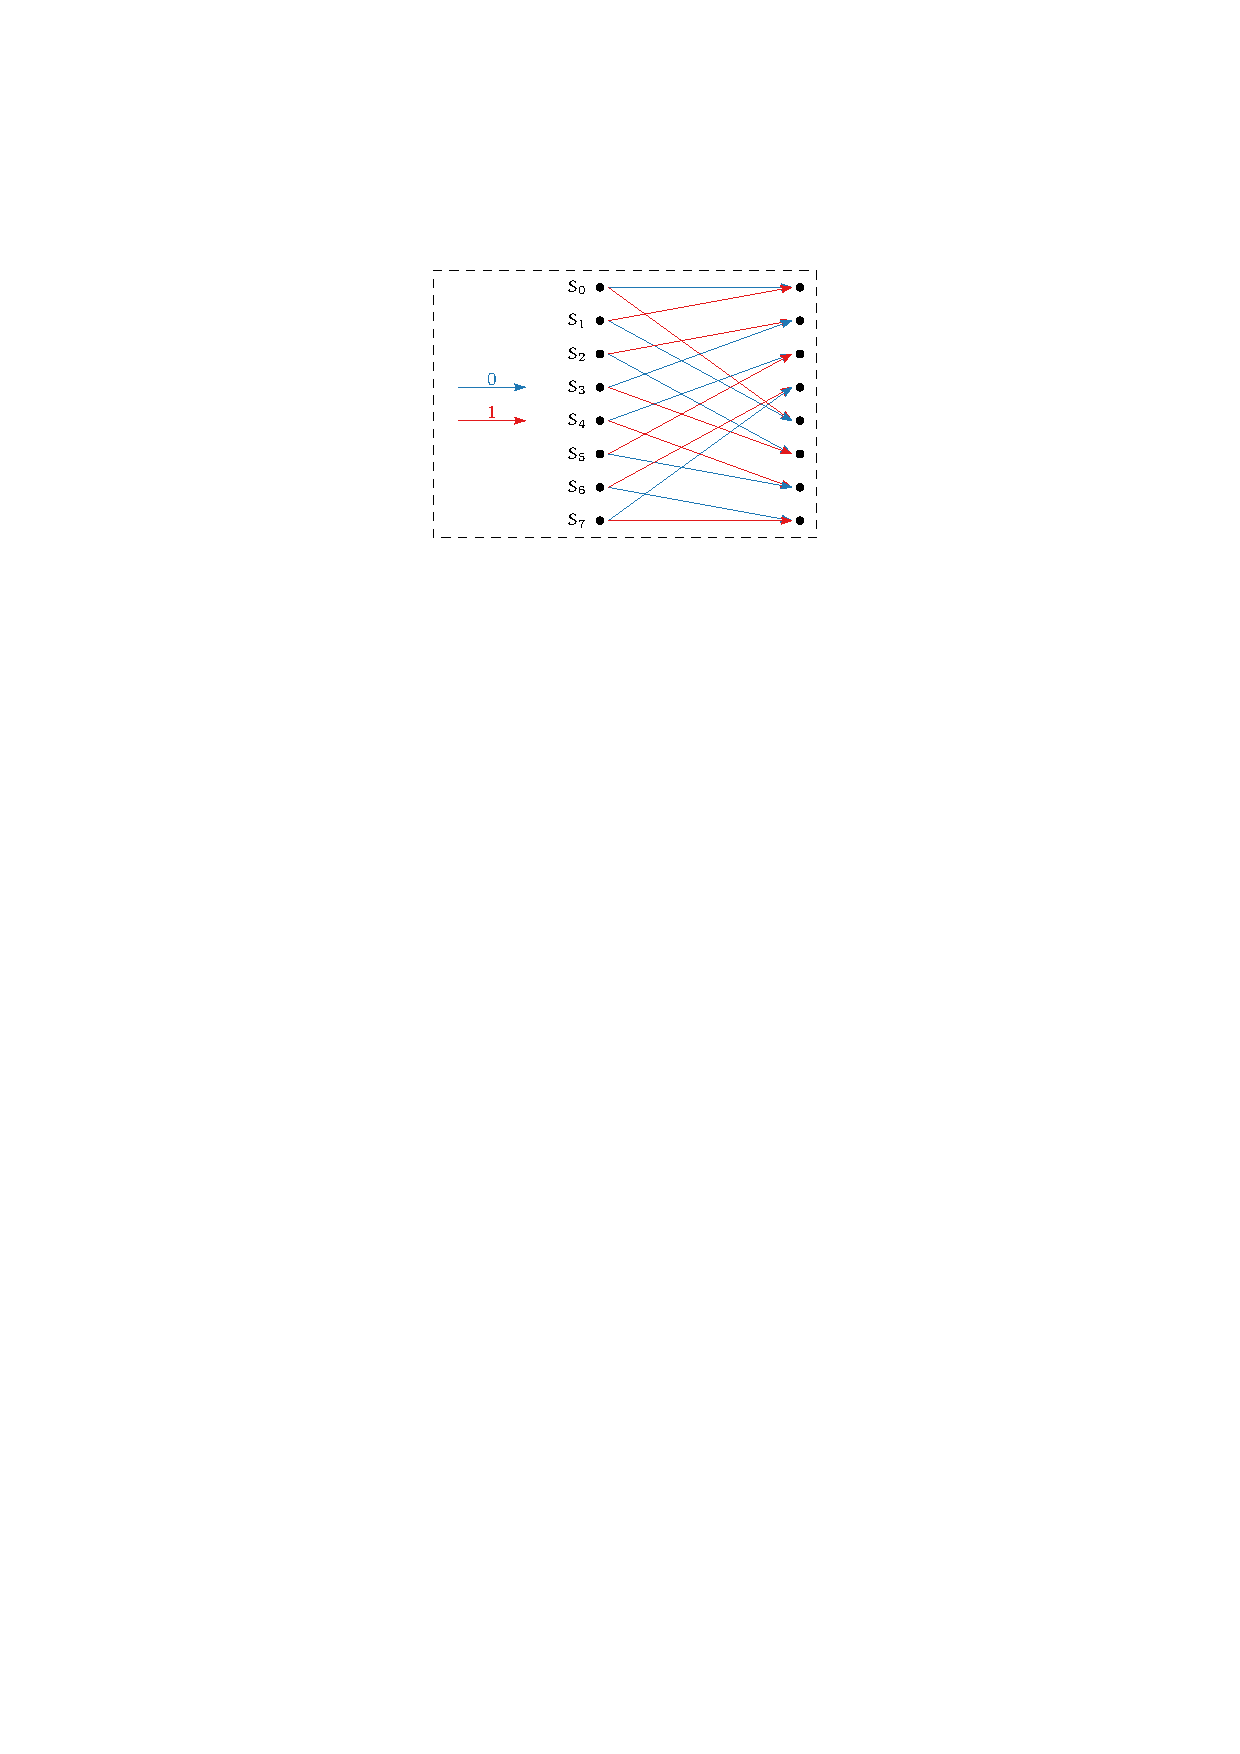
\includegraphics[width=0.48\textwidth]{main/ch1_fig/lte}
			\label{sub:lte}
		}	    
		\subfloat[DVB-RCS]{
			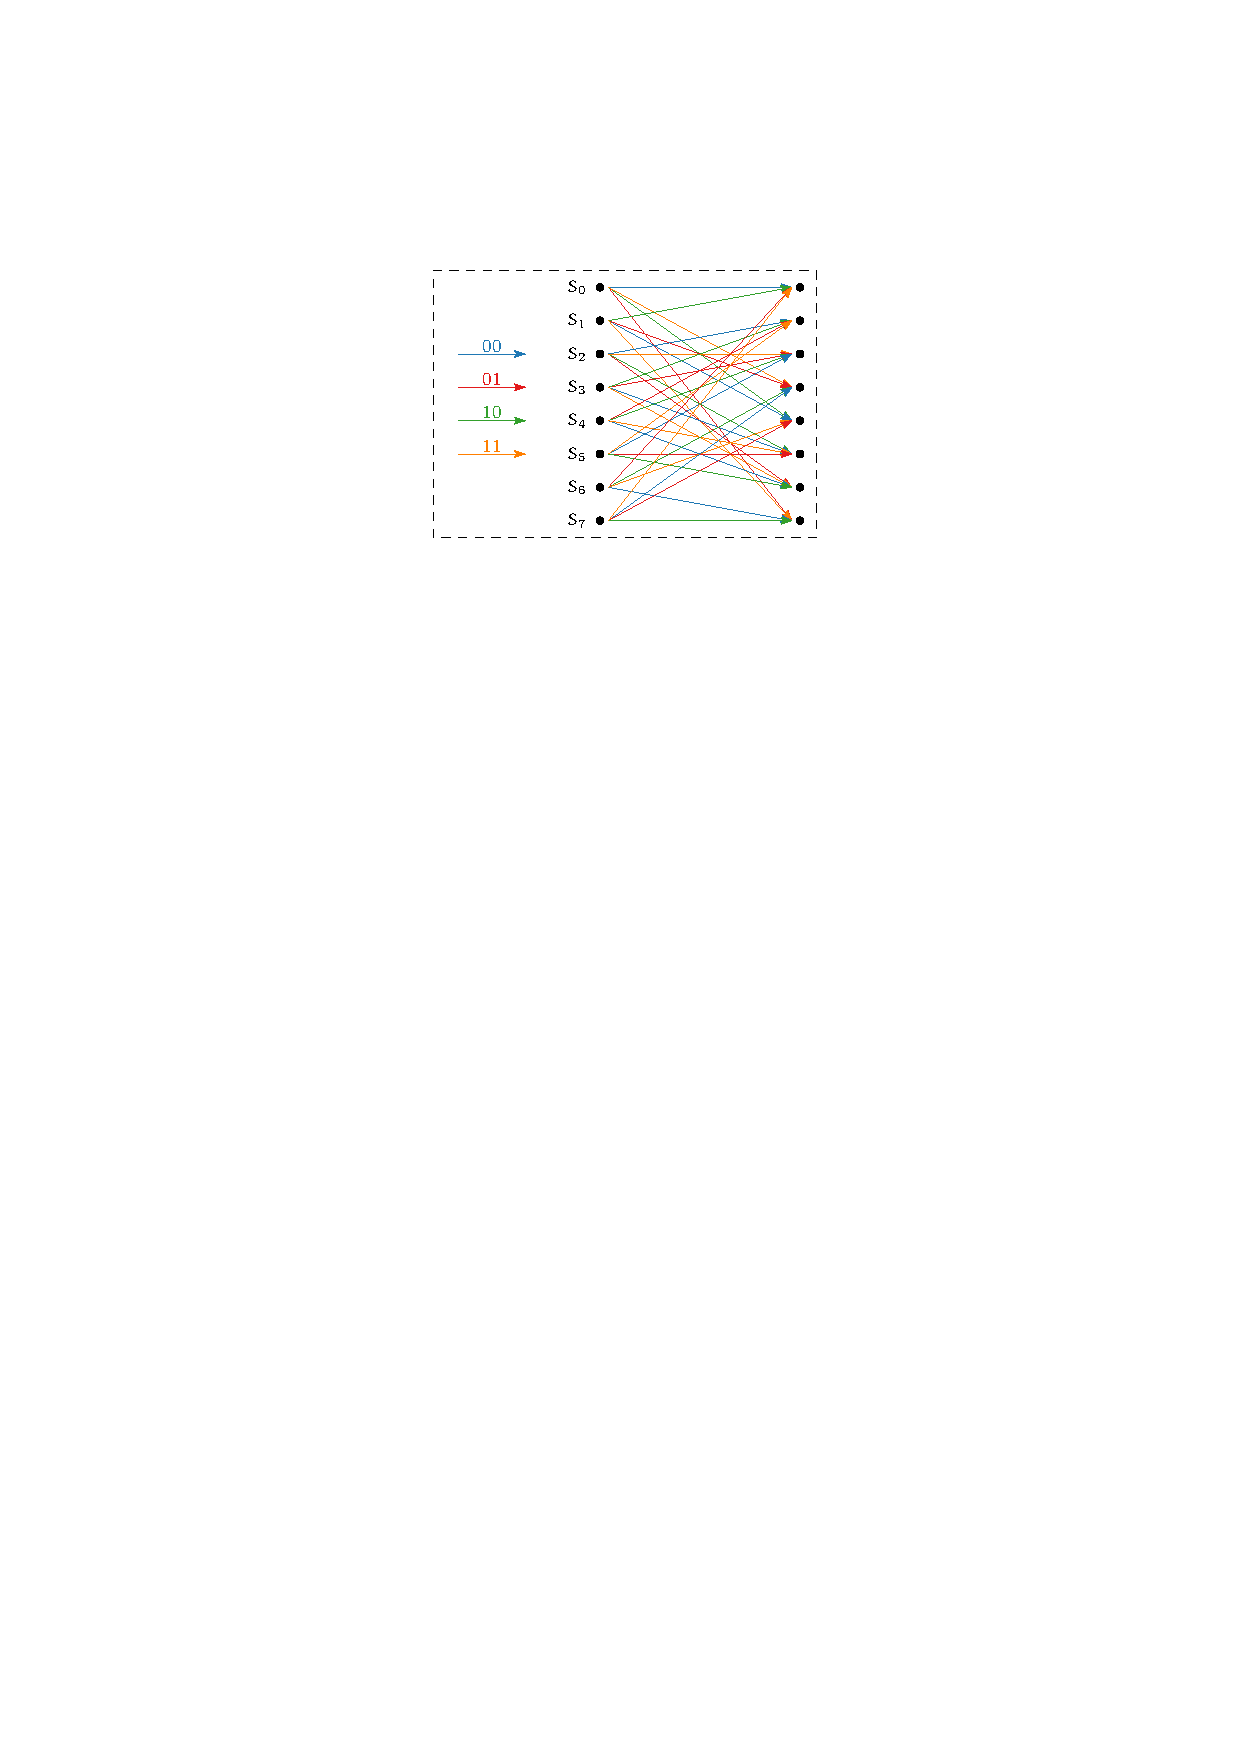
\includegraphics[width=0.48\textwidth]{main/ch1_fig/dvbrcs.pdf}
			\label{sub:dvbrcs}
		}
																																																																																																																																										
		\subfloat[CCSDS]{
			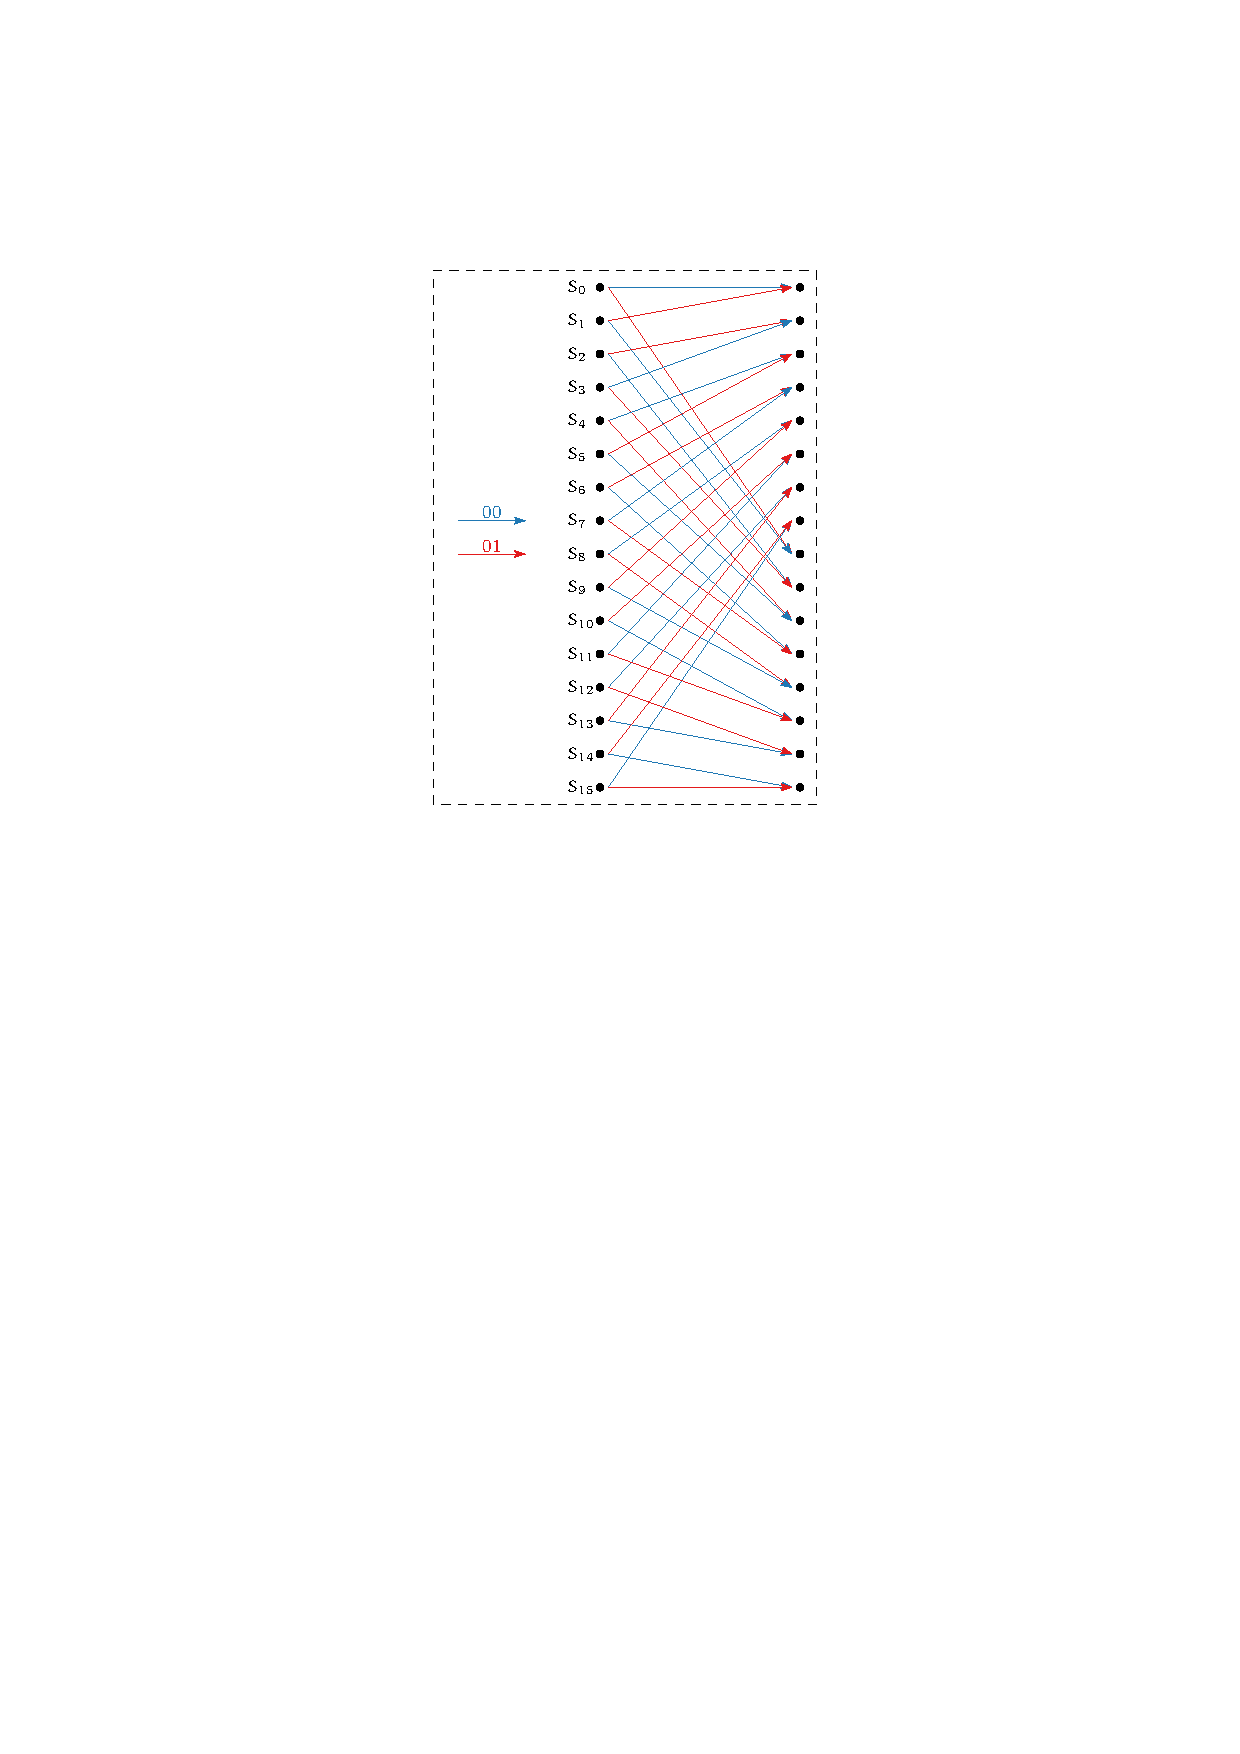
\includegraphics[width=0.48\textwidth]{main/ch1_fig/ccsds}
			\label{sub:ccsds}
		}
		\subfloat[DVB-RCS2]{
			\includegraphics[width=0.48\textwidth]{main/ch1_fig/dvbrcs2_3.pdf}
			\label{sub:dvbrcs2}
		}
		\caption{Treillis associés aux codeurs RSC élémentaires des turbo codes du tableau \ref{tab:std}}
		\label{fig:treillisstd}
	\end{center}
\end{figure}

% \begin{figure}[h!]
% 	\begin{center}
% 		\subfloat[LTE R=1/3]{
% 			%!TEX root = ../../../my_thesis.tex
\begin{tikzpicture}
	\begin{semilogyaxis}[footnotesize, width=0.8\linewidth, height=0.6\linewidth,    
			xmin=0, xmax=3, xtick={0,0.4,...,3.0},
			%ymin=2e-6,  ymax=0.11,
			xlabel=$E_b/N_0 \text{(dB)}$, ylabel=FER,  grid=both, grid style={gray!30},
		tick align=outside, tickpos=left, legend pos=north east]
																				
		\addplot[mark=o,Paired-1]  table [x=SNR, y=FER] {main/ch1_fig/std/lte13_528.dat}; 
		\addplot[mark=diamond,Paired-3]  table [x=SNR, y=FER] {main/ch1_fig/std/lte13_1504.dat}; 
		\addplot[mark=square,Paired-5]  table [x=SNR, y=FER] {main/ch1_fig/std/lte13_2048.dat}; 
		\addplot[mark=triangle,Paired-7]  table [x=SNR, y=FER] {main/ch1_fig/std/lte13_6144.dat}; 
																						
																														
		\legend{K=528, K=1504, K=2048, K=6144}
																														
	\end{semilogyaxis}
\end{tikzpicture}  
% 			\label{sub:lte}
% 		}	    
% 		\subfloat[LTE R=4/5]{
% 			%!TEX root = ../../../my_thesis.tex
\begin{tikzpicture}
	\begin{semilogyaxis}[footnotesize, width=0.9\linewidth, height=0.6\linewidth,    
			xmin=2.0, xmax=5, xtick={2,2.4,...,5.0},
			%ymin=2e-6,  ymax=0.11,
			xlabel=$E_b/N_0 \text{(dB)}$, ylabel=FER,  grid=both, grid style={gray!30},
			/pgfplots/table/ignore chars={|},
		    tick align=outside, tickpos=left, legend pos=north east]
																																														
														
		\addplot[mark=o,       Paired-1, restrict x to domain=2.0:4.4,semithick] table [x=Eb/N0, y=FER] {main/ch1_fig/std/aff3ct/528_45.txt};
		\addplot[mark=diamond, Paired-3, restrict x to domain=2.0:4.4,semithick] table [x=Eb/N0, y=FER] {main/ch1_fig/std/aff3ct/1504_45.txt}; 
		\addplot[mark=square,  Paired-5, restrict x to domain=2.0:4.4,semithick] table [x=Eb/N0, y=FER] {main/ch1_fig/std/aff3ct/2048_45.txt}; 
		\addplot[mark=triangle,Paired-7, restrict x to domain=2.0:4.4,semithick] table [x=Eb/N0, y=FER] {main/ch1_fig/std/aff3ct/6144_45.txt}; 		
																																																									
		\legend{K=528, K=1504, K=2048, K=6144}
																																																									
	\end{semilogyaxis}
\end{tikzpicture}  
% 			\label{sub:dvbrcs}
% 		}
																																																																																																																																										
% 		\subfloat[DVB-RSC K=220]{
% 			%!TEX root = ../../../my_thesis.tex
\begin{tikzpicture}
	\begin{semilogyaxis}[footnotesize, width=0.8\linewidth, height=0.6\linewidth,    
			xmin=0, xmax=3, xtick={0,0.4,...,3.0},
			%ymin=2e-6,  ymax=0.11,
			xlabel=$E_b/N_0 \text{(dB)}$, ylabel=FER,  grid=both, grid style={gray!30},
		tick align=outside, tickpos=left, legend pos=north east]
																				
		\addplot[mark=o,Paired-1]  table [x=SNR, y=FER] {main/ch1_fig/std/lte13_528.dat}; 
		\addplot[mark=diamond,Paired-3]  table [x=SNR, y=FER] {main/ch1_fig/std/lte13_1504.dat}; 
		\addplot[mark=square,Paired-5]  table [x=SNR, y=FER] {main/ch1_fig/std/lte13_2048.dat}; 
		\addplot[mark=triangle,Paired-7]  table [x=SNR, y=FER] {main/ch1_fig/std/lte13_6144.dat}; 
																						
																														
		\legend{K=528, K=1504, K=2048, K=6144}
																														
	\end{semilogyaxis}
\end{tikzpicture}  
% 			\label{sub:ccsds}
% 		}
% 		\subfloat[DVB-RSC K=752]{
% 			%!TEX root = ../../../my_thesis.tex
\begin{tikzpicture}
	\begin{semilogyaxis}[footnotesize, width=0.8\linewidth, height=0.6\linewidth,    
			xmin=0, xmax=3, xtick={0,0.4,...,3.0},
			%ymin=2e-6,  ymax=0.11,
			xlabel=$E_b/N_0 \text{(dB)}$, ylabel=FER,  grid=both, grid style={gray!30},
		tick align=outside, tickpos=left, legend pos=north east]
																				
		\addplot[mark=o,Paired-1]  table [x=SNR, y=FER] {main/ch1_fig/std/lte13_528.dat}; 
		\addplot[mark=diamond,Paired-3]  table [x=SNR, y=FER] {main/ch1_fig/std/lte13_1504.dat}; 
		\addplot[mark=square,Paired-5]  table [x=SNR, y=FER] {main/ch1_fig/std/lte13_2048.dat}; 
		\addplot[mark=triangle,Paired-7]  table [x=SNR, y=FER] {main/ch1_fig/std/lte13_6144.dat}; 
																						
																														
		\legend{K=528, K=1504, K=2048, K=6144}
																														
	\end{semilogyaxis}
\end{tikzpicture}  
% 			\label{sub:dvbrcs2}
% 		}
																																																																																																																																								
% 		\subfloat[CCSDS]{
% 			%!TEX root = ../../../my_thesis.tex
\begin{tikzpicture}
	\begin{semilogyaxis}[footnotesize, width=0.8\linewidth, height=0.6\linewidth,    
			xmin=0, xmax=3, xtick={0,0.4,...,3.0},
			%ymin=2e-6,  ymax=0.11,
			xlabel=$E_b/N_0 \text{(dB)}$, ylabel=FER,  grid=both, grid style={gray!30},
		tick align=outside, tickpos=left, legend pos=north east]
																				
		\addplot[mark=o,Paired-1]  table [x=SNR, y=FER] {main/ch1_fig/std/lte13_528.dat}; 
		\addplot[mark=diamond,Paired-3]  table [x=SNR, y=FER] {main/ch1_fig/std/lte13_1504.dat}; 
		\addplot[mark=square,Paired-5]  table [x=SNR, y=FER] {main/ch1_fig/std/lte13_2048.dat}; 
		\addplot[mark=triangle,Paired-7]  table [x=SNR, y=FER] {main/ch1_fig/std/lte13_6144.dat}; 
																						
																														
		\legend{K=528, K=1504, K=2048, K=6144}
																														
	\end{semilogyaxis}
\end{tikzpicture}  
% 			\label{sub:ccsds}
% 		}
% 		\subfloat[DVB-RSC2]{
% 			%!TEX root = ../../../my_thesis.tex
\begin{tikzpicture}
	\begin{semilogyaxis}[footnotesize, width=0.8\linewidth, height=0.6\linewidth,    
			xmin=0, xmax=3, xtick={0,0.4,...,3.0},
			%ymin=2e-6,  ymax=0.11,
			xlabel=$E_b/N_0 \text{(dB)}$, ylabel=FER,  grid=both, grid style={gray!30},
		tick align=outside, tickpos=left, legend pos=north east]
																				
		\addplot[mark=o,Paired-1]  table [x=SNR, y=FER] {main/ch1_fig/std/lte13_528.dat}; 
		\addplot[mark=diamond,Paired-3]  table [x=SNR, y=FER] {main/ch1_fig/std/lte13_1504.dat}; 
		\addplot[mark=square,Paired-5]  table [x=SNR, y=FER] {main/ch1_fig/std/lte13_2048.dat}; 
		\addplot[mark=triangle,Paired-7]  table [x=SNR, y=FER] {main/ch1_fig/std/lte13_6144.dat}; 
																						
																														
		\legend{K=528, K=1504, K=2048, K=6144}
																														
	\end{semilogyaxis}
\end{tikzpicture}  
% 			\label{sub:dvbrcs2}
% 		}
% 		\caption{Taux d'erreur trame pour les différents standards et pour différentes configurations. Décodage par l'algorithme EML-MAP effectuant 8 itérations, critère d’arrêt génie}
% 		\label{fig:ferstd}
% 	\end{center}
% \end{figure}

\begin{figure}[h]
	\begin{center}
		\subfloat[LTE R=1/3]{
			%!TEX root = ../../../my_thesis.tex
\begin{tikzpicture}
	\begin{semilogyaxis}[footnotesize, width=0.8\linewidth, height=0.6\linewidth,    
			xmin=0, xmax=3, xtick={0,0.4,...,3.0},
			%ymin=2e-6,  ymax=0.11,
			xlabel=$E_b/N_0 \text{(dB)}$, ylabel=FER,  grid=both, grid style={gray!30},
		tick align=outside, tickpos=left, legend pos=north east]
																				
		\addplot[mark=o,Paired-1]  table [x=SNR, y=FER] {main/ch1_fig/std/lte13_528.dat}; 
		\addplot[mark=diamond,Paired-3]  table [x=SNR, y=FER] {main/ch1_fig/std/lte13_1504.dat}; 
		\addplot[mark=square,Paired-5]  table [x=SNR, y=FER] {main/ch1_fig/std/lte13_2048.dat}; 
		\addplot[mark=triangle,Paired-7]  table [x=SNR, y=FER] {main/ch1_fig/std/lte13_6144.dat}; 
																						
																														
		\legend{K=528, K=1504, K=2048, K=6144}
																														
	\end{semilogyaxis}
\end{tikzpicture}  
			\label{sub:lte13}
		}	   

		\subfloat[LTE R=4/5]{
			%!TEX root = ../../../my_thesis.tex
\begin{tikzpicture}
	\begin{semilogyaxis}[footnotesize, width=0.9\linewidth, height=0.6\linewidth,    
			xmin=2.0, xmax=5, xtick={2,2.4,...,5.0},
			%ymin=2e-6,  ymax=0.11,
			xlabel=$E_b/N_0 \text{(dB)}$, ylabel=FER,  grid=both, grid style={gray!30},
			/pgfplots/table/ignore chars={|},
		    tick align=outside, tickpos=left, legend pos=north east]
																																														
														
		\addplot[mark=o,       Paired-1, restrict x to domain=2.0:4.4,semithick] table [x=Eb/N0, y=FER] {main/ch1_fig/std/aff3ct/528_45.txt};
		\addplot[mark=diamond, Paired-3, restrict x to domain=2.0:4.4,semithick] table [x=Eb/N0, y=FER] {main/ch1_fig/std/aff3ct/1504_45.txt}; 
		\addplot[mark=square,  Paired-5, restrict x to domain=2.0:4.4,semithick] table [x=Eb/N0, y=FER] {main/ch1_fig/std/aff3ct/2048_45.txt}; 
		\addplot[mark=triangle,Paired-7, restrict x to domain=2.0:4.4,semithick] table [x=Eb/N0, y=FER] {main/ch1_fig/std/aff3ct/6144_45.txt}; 		
																																																									
		\legend{K=528, K=1504, K=2048, K=6144}
																																																									
	\end{semilogyaxis}
\end{tikzpicture}  
			\label{sub:lte45}
		}
																																																																																																																																									
		\caption{Taux d'erreur trame pour le standard LTE pour deux rendements et différentes tailles de trame. Décodage par l'algorithme EML-MAP effectuant 8 itérations}
		\label{fig:ferstdlte}
	\end{center}
\end{figure}

\begin{figure}[h]
	\begin{center}
		\subfloat[DVB-RCS - K=220]{
			%!TEX root = ../../../my_thesis.tex
\begin{tikzpicture}
	\begin{semilogyaxis}[footnotesize, width=0.9\linewidth, height=0.6\linewidth,    
			xmin=0, xmax=3, xtick={0,0.4,...,3.0},
			ymin=1e-7,  ymax=1,
			xlabel=$E_b/N_0 \text{(dB)}$, ylabel=FER,  grid=both, grid style={gray!30},
		tick align=outside, tickpos=left, legend pos=north east]
																				
	%	\addplot[mark=o,Paired-1]  table [x=SNR, y=FER] {main/ch1_fig/std/lte13_528.dat}; 
	%	\addplot[mark=diamond,Paired-3]  table [x=SNR, y=FER] {main/ch1_fig/std/lte13_1504.dat}; 
	%	\addplot[mark=square,Paired-5]  table [x=SNR, y=FER] {main/ch1_fig/std/lte13_2048.dat}; 
	%	\addplot[mark=triangle,Paired-7]  table [x=SNR, y=FER2] {main/ch1_fig/std/lte13_6144.dat}; 
																						
																														
	%	\legend{K=528, K=1504, K=2048, K=6144}

	\node[Paired-5,above,rotate=30] at (axis cs:1.5,10e-4){\Huge Simulations en cours};																														
	\end{semilogyaxis}
\end{tikzpicture}  
			\label{sub:dvbrcs220}
		}	   

		\subfloat[DVB-RCS - K=752]{
			%!TEX root = ../../../my_thesis.tex
\begin{tikzpicture}
	\begin{semilogyaxis}[footnotesize, width=0.9\linewidth, height=0.6\linewidth,    
			xmin=0, xmax=3, xtick={0,0.4,...,3.0},
			ymin=1e-7,  ymax=1,
			xlabel=$E_b/N_0 \text{(dB)}$, ylabel=FER,  grid=both, grid style={gray!30},
		tick align=outside, tickpos=left, legend pos=north east]
																				
	%	\addplot[mark=o,Paired-1]  table [x=SNR, y=FER] {main/ch1_fig/std/lte13_528.dat}; 
	%	\addplot[mark=diamond,Paired-3]  table [x=SNR, y=FER] {main/ch1_fig/std/lte13_1504.dat}; 
	%	\addplot[mark=square,Paired-5]  table [x=SNR, y=FER] {main/ch1_fig/std/lte13_2048.dat}; 
	%	\addplot[mark=triangle,Paired-7]  table [x=SNR, y=FER2] {main/ch1_fig/std/lte13_6144.dat}; 
																						
																														
	%	\legend{K=528, K=1504, K=2048, K=6144}

	\node[Paired-5,above,rotate=30] at (axis cs:1.5,10e-4){\Huge Simulations en cours};																														
	\end{semilogyaxis}
\end{tikzpicture}  
			\label{sub:dvbrcs752}
		}
																																																																																																																																									
		\caption{Taux d'erreur trame pour le standard DVB-RCS pour plusieurs rendements et deux tailles de trame. Décodage par l'algorithme EML-MAP effectuant 8 itérations}
		\label{fig:ferstdDVB1}
	\end{center}
\end{figure}


\begin{figure}[h]
\centering
			%!TEX root = ../../../my_thesis.tex
\begin{tikzpicture}
	\begin{semilogyaxis}[footnotesize, width=0.9\linewidth, height=0.6\linewidth,    
			xmin=0, xmax=3, xtick={0,0.4,...,3.0},
			ymin=1e-7,  ymax=1,
			xlabel=$E_b/N_0 \text{(dB)}$, ylabel=FER,  grid=both, grid style={gray!30},
		tick align=outside, tickpos=left, legend pos=north east]
																				
	%	\addplot[mark=o,Paired-1]  table [x=SNR, y=FER] {main/ch1_fig/std/lte13_528.dat}; 
	%	\addplot[mark=diamond,Paired-3]  table [x=SNR, y=FER] {main/ch1_fig/std/lte13_1504.dat}; 
	%	\addplot[mark=square,Paired-5]  table [x=SNR, y=FER] {main/ch1_fig/std/lte13_2048.dat}; 
	%	\addplot[mark=triangle,Paired-7]  table [x=SNR, y=FER2] {main/ch1_fig/std/lte13_6144.dat}; 
																						
																														
	%	\legend{K=528, K=1504, K=2048, K=6144}

	\node[Paired-5,above,rotate=30] at (axis cs:1.5,10e-4){\Huge Simulations en cours};																														
	\end{semilogyaxis}
\end{tikzpicture}  	
		\caption{Taux d'erreur trame pour le standard CCSDS pour deux rendements et deux tailles de trame. Décodage par l'algorithme EML-MAP effectuant 8 itérations, critère d’arrêt génie}
		\label{fig:ferstdCCSDS}
\end{figure}

\begin{figure}[h]
\centering
			%!TEX root = ../../../my_thesis.tex
\begin{tikzpicture}
	\begin{semilogyaxis}[footnotesize, width=0.9\linewidth, height=0.6\linewidth,    
			xmin=0, xmax=3, xtick={0,0.4,...,3.0},
			ymin=1e-7,  ymax=1,
			xlabel=$E_b/N_0 \text{(dB)}$, ylabel=FER,  grid=both, grid style={gray!30},
		tick align=outside, tickpos=left, legend pos=north east]
																				
	%	\addplot[mark=o,Paired-1]  table [x=SNR, y=FER] {main/ch1_fig/std/lte13_528.dat}; 
	%	\addplot[mark=diamond,Paired-3]  table [x=SNR, y=FER] {main/ch1_fig/std/lte13_1504.dat}; 
	%	\addplot[mark=square,Paired-5]  table [x=SNR, y=FER] {main/ch1_fig/std/lte13_2048.dat}; 
	%	\addplot[mark=triangle,Paired-7]  table [x=SNR, y=FER2] {main/ch1_fig/std/lte13_6144.dat}; 
																						
																														
	%	\legend{K=528, K=1504, K=2048, K=6144}

	\node[Paired-5,above,rotate=30] at (axis cs:1.5,10e-4){\Huge Simulations en cours};																														
	\end{semilogyaxis}
\end{tikzpicture}  	
		\caption{Taux d'erreur trame pour le standard DVB-RCS2. Décodage par l'algorithme EML-MAP effectuant 8 itérations, critère d’arrêt génie}
		\label{fig:ferstdDVB2}
\end{figure}

\clearpage
A partir des Figures \ref{fig:ferstdlte} à \ref{fig:ferstdDVB2}, nous pouvons remarquer que les performances de décodage des turbo codes peuvent être différenciées selon trois régions :
\begin{itemize}
	\item La première zone, correspondant aux faibles valeurs de SNR est nommé \og zone de non convergence \fg. Pour de tels valeurs de SNR, le système codé peut-être moins performant que le système de transmission codée.
	\item Passé le seuil de convergence, une faible augmentation du SNR implique une baisse significative du taux d'erreur. Cette zone est nommée \og waterfall region \fg  en anglais.
	\item Enfin, dans la région du \og plancher d'erreur \fg, la courbe de performance s’aplatit : le taux d'erreur baisse légèrement lorsque le SNR augmente.
\end{itemize}

Afin d'obtenir des codes approchant la capacité du canal, il est nécessaire que le seuil de convergence soit atteint au plus tôt. La méthode du diagramme EXIT \cite{exitchart} permet de caractériser et de prévoir ce seuil. 
%Cependant, cette méthode n'est pas détaillée dans ce manuscrit.

Dans la zone de convergence, l'augmentation du nombre d'itérations améliore les performances. En revanche, dans la zone du plancher d'erreur, seulement quelques itérations sont nécessaires et les suivantes n'amènent qu'un gain marginal en terme de performances.

Le plancher d'erreur peut limiter l'utilisation des turbo codes pour des applications nécessitant de très faibles taux d'erreur. Comme cette zone de gain asymptotique est essentiellement influencée par la distance minimale de Hamming du code, le problème du plancher d'erreurs est discuté dans la section suivante.

\subsection{Le problème du plancher d'erreurs}

\subsubsection{Performances asymptotiques sur canal BI-AWGN}
Nous avons préalablement expliqué qu'en raison de l'étape d'entrelacement un décodage ML de turbo codes n'est pas possible. Ainsi, les méthodes de décodage itératives employées sont sous-optimales. Cependant elles approchent les performances ML pour des valeurs de SNR moyennes à élevées.
Nous allons donc dans cette section estimer les performances d'un décodeur ML pour un turbo code utilisé sur le canal BI-AWGN.

Puisque les codes constituant et l'entrelaceur d'un turbo code sont linéaires, lui-même l'est sous réserve d'omettre la séquence de terminaison. Cette propriété de linéarité combinée à la symétrie du canal considéré implique que la probabilité d'erreur sachant qu'un certain mot de code $\mathbf{c}$ a été émis est la même que si un autre mot de code $\mathbf{c'}$ était transmis. Ceci permet de simplifier l'analyse en considérant que le mot de code tout à zéro ($\mathbf{0}$) est transmis.

Ainsi, la probabilité qu'un mot soit erroné vaut : 
\begin{align}\label{eq:err}
	P_{cw} & = P(erreur~|~\mathbf{0}) \notag                                                             \\
	       & = P( \decide\limits_{\mathbf{\hat{c}}\neq \mathbf{0}} \mathbf{\hat{c}}~|~\mathbf{0}) \notag \\
	       & \le \sum\limits_{\mathbf{\hat{c}}\neq \mathbf{0}}P( \decide \mathbf{\hat{c}}~|~\mathbf{0}). 
\end{align}
Ceci correspond au fait que le décodeur choisisse le mot de code $\mathbf{\hat{c}}$ alors que $\mathbf{0}$ est transmis.

Soit $m(\mathbf{c})$ la représentation après transmission du mot de code $\mathbf{c}$. Nous pouvons alors écrire $m(\mathbf{0}) = (\sqrt{E_c},\sqrt{E_c},...,\sqrt{E_c})$, avec $E_c = RE_b$.\\
Posons $P_w$ la probabilité que le bruit blanc gaussien implique que le vecteur reçu $\mathbf{r}$ soit plus près de  $m(\mathbf{\hat{c}})$ que de $m(\mathbf{0})$, avec $m(\mathbf{\hat{c}}) = (\sqrt{E_c},-\sqrt{E_c},...,\sqrt{E_c})$ et $w$ le nombre de positions différant de $m(\mathbf{0})$.

Ainsi, $m(\mathbf{\hat{c}})$ et $m(\mathbf{0})$ sont séparés par la distance (Euclidienne) $d_E = 2\sqrt{wE_c} = 2\sqrt{wRE_b}$. Introduisons la fonction $Q(x)$ représentant la probabilité qu'une variable aléatoire Gaussienne ait une valeur plus grande que $x$ fois l'écart type autour de la moyenne ($x=\frac{y_\mu}{\sigma}$). Nous pouvons alors exprimer $P_w$ en utilisant cette fonction puisque $P_w$ représente la probabilité que le bruit en direction de $\mathbf{\hat{c}}$ soit plus grand que $\frac{d_E}{2} = \sqrt{wRE_b}$ : 
\begin{equation}\label{eq:perr}
	P_w = Q\left(\frac{d_E}{2\sigma}\right) = Q\left(\frac{\sqrt{wRE_b}}{\sigma}\right) = Q\left(\sqrt{\frac{2wRE_b}{N_0}}\right).  
\end{equation} 

Or, en posant $A_w$ la multiplicité ou le nombre de mots de code de poids $w$, nous pouvons réécrire l'équation \ref{eq:err} de la sorte : 
\[P_{cw} \le \sum\limits_w A_wP_w.\]
En reprenant l'équation \ref{eq:perr}, nous pouvons finalement écrire :
\begin{equation} \label{eq:uboundfer}
	P_{cw} \le \sum\limits_w A_w Q\left(\sqrt{\frac{2wRE_b}{N_0}}\right)
\end{equation}
Cette équation donne donc une borne supérieure quant à la probabilité d'erreur mot en utilisant un décodeur ML. En découle son équivalent binaire exprimé par :
\begin{equation} \label{eq:uboundfer}
	P_{b} \le \sum\limits_w \frac{W_w}{K} Q\left(\sqrt{\frac{2wRE_b}{N_0}}\right)
\end{equation} 
où $W_w$ est la somme des poids de Hamming des $A_w$ séquences binaires générant  des mots de codes de poids de Hamming $w$.
	
Ainsi, selon les valeurs ($w,A_w,W_w$) associées à un code, nous pouvons exprimer des bornes quant aux performances obtenues avec un décodeur ML. Les valeurs ($w,A_w,W_w$) se nomment spectre de distance du code et les bornes sont les \emph{bornes de l'union}. Or, il s'avère qu'en utilisant un décodeur sous-optimal itératif, les performances approchent les bornes dans le régime asymptotique.
	
C'est pourquoi, de nombreux travaux de recherche ont porté sur l'extraction des spectres de distance afin de prévoir le comportement asymptotique d'un turbo code.
	
\subsubsection{Méthodes d'obtention du spectre de distance de turbo codes}\label{seq:spectre}
Les premières méthodes visant à obtenir le spectre de distance sont basées sur des approches par force brute \cite{illuminating}. Leur principe est de considérer toutes les séquences possibles pour le premier codeur constitutif, de les entrelacer et de les coder avec le second codeur constitutif afin d'obtenir la distance du code. Cependant, pour des distances minimales conséquentes, cette recherche devient impossible à mener.
	
En 2001, un algorithme basé sur l'utilisation de sous codes contraints a été proposé par Garello \textit{et al.} \cite{garellodfree}. Cet algorithme permet de déterminer exactement les premiers termes du spectre. Cependant, lorsque la taille du code et la distance minimale sont conséquentes, le temps de calcul est prohibitif rendant cet algorithme difficile à exploiter.
	
Ainsi, plusieurs techniques ont été proposées qui se basant pas sur sur la capacité de correction du décodeur plutôt que sur les propriétés du code. En 2002, Berrou \textit{et al.} ont proposé une méthode rapide basée sur la capacité d'un décodeur à compenser l'insertion d'un événement d'erreur \cite{eim}. Son principe est d'insérer une impulsion croissante $A_i$ dans le mot de code tout-à-zéro, ce pour toutes les positions $i$, ($0\le i \le K-1$). Lorsque l'impulsion est suffisamment grande, le décodeur ne converge plus vers le mot de code $\mathbf{0}$ (tout à zéro). Posons $A_i^*$ l'amplitude maximale de l’impulsion à la position $i$ ne mettant pas en défaut le décodeur. Il a alors été montré que dans le cas d'un décodeur ML, la distance impulsionnelle définie par $d_imp = \min\limits_i (A_i)$ est aussi la distance minimale du code. Puisque le décodage des turbo codes n'est pas ML, la véritable $d_{min}$ n'est pas toujours obtenue par cette méthode. Il a été constaté que cette méthode est plutôt pessimiste mais néanmoins, des distances plus grandes que la vraie $d_{min}$ ont été trouvées \cite{yocComparisonMethods}.
	
En 2004, Garello \textit{et al.} ont proposé une méthode similaire à la précédente \cite{garelloAllZero}. Dans celle-ci, l'impulsion d'erreur empêche le décodeur de converger vers le mot de code $\mathbf{0}$. Il converge donc vers une séquence d'entrée non-nulle. En encodant cette séquence d'entrée, un mot de code non-nul est obtenu. Le poids de Hamming de ce mot de code est alors une borne supérieure de la distance minimale du code. Cependant, cette méthode propose des résultats probants uniquement pour des codes possédant de faibles $d_{min}$ \cite{yocComparisonMethods}.
	
Enfin, en 2005, Crozier \textit{et al.} ont développé deux méthodes améliorées, découlant de la précédente \cite{crozierDIM}. Une première impulsion est placée à une position $i$ dans la partie systématique du mot de code. Une seconde est ajoutée à une position $j$. Ensuite le décodage est mené et les distances et multiplicités associées sont relevées de la même manière que dans \cite{garelloAllZero}. Les auteurs considèrent que placer la seconde impulsion dans la zone $\llbracket i; i+2D\rrbracket$, avec D la distance minimale du code estimée est suffisant. Cependant, dans \cite{yocComparisonMethods}, il est précisé que la fiabilité de cette méthode est accrue si $j \in \llbracket i; K-1\rrbracket$. Pis encore, selon nos expérimentations, dans le cas de turbo codes non circulaires, afin d’approcher au plus près les résultats fournis par la méthode \cite{garellodfree}, imposer $i \in \llbracket 0; K-1\rrbracket$ et $j \in \llbracket i; N\rrbracket$ semblent offrir le meilleur compromis.
	
\paragraph*{Exemples de prévision du plancher d'erreur}
En utilisant la méthode de la double impulsion de Crozier \cite{crozierDIM} ou la méthode utilisant les sous-codes contraints de Garello \cite{garellodfree}, nous pouvons calculer les spectres de distance pour les différents turbo codes standardisés.

Le tableau \ref{tab:spectre} présente les premiers termes du spectre de distance pour le turbo code du standard LTE pour $K \in \{528; 2048; 6144\}$ et $R=1/3$. Nous pouvons remarquer que les multiplicités sont faibles et que les distances minimales sont globalement croissantes avec $K$.

% \begin{table}[]
% 	\centering
% 	\caption{Spectre de sitantce pour 3 turbo codes du standard LTE}
% 	\label{tab:spectre}
% 	\resizebox{\textwidth}{!}{%
% 		\begin{tabular}{rlllllllllllllll}
% 			\toprule
% 			\textbf{K}    & \multicolumn{15}{c}{d/Ad/Wd}                                                                                                                                  \\
% 			\cmidrule(l){1-1}
% 			
% 			\multirow{2}{*}{\textbf{528}}  & 23/1/1 & 24/1/2 & 25/1/3 & 27/3/9 & 28/3/6 & 29/6/16 & 31/8/28 & 32/5/18 & 33/16/54 & 34/12/38 & 35/20/80 & 36/24/92 & 37/163/527 & 38/1019/6030 & 39/163/527 \\
% 			\textbf{2048} & 27/1/1 & 28/2/4 & 29/1/3 & 30/1/2 & 31/3/9 & 33/2/6  & 34/1/4  & 35/2/6  & 36/1/4   & 37/3/8   & 38/5/16  & 39/12/18 & 40/6/24    & 41/16/62     & 43/21/95   \\
% 			\textbf{6144} & 26/1/2 &        &        &        &        &         &         &         &          &          &          &          &            &              &            \\        
% 			\bottomrule
% 		\end{tabular}}
% \end{table}

\begin{table}[]
\centering
\caption{Spectre de distance pour trois turbo codes du standard LTE}
\label{tab:spectre}
\resizebox{\textwidth}{!}{%
\begin{tabular}{rllllllll}
\toprule
\textbf{K}                                         & \multicolumn{8}{c}{$\mathbf{d/A_d/W_d}$}                                                                 \\
\cmidrule(lr){1-1}
			\cmidrule(lr){2-9}
\multirow{2}{*}{\textbf{528}}                      & 23/1/1 & 24/1/2   & 25/1/3   & 27/3/9   & 28/3/6   & 29/6/16    & 31/8/28      & 32/5/18    \\
                                          &        & 33/16/54 & 34/12/38 & 35/20/80 & 36/24/92 & 37/163/527 & 38/1019/6030 & 39/163/527 \\ \cdashlinelr{2-9}
\multicolumn{1}{c}{\multirow{2}{*}{\textbf{2048}}} & 27/1/1 & 28/2/4   & 29/1/3   & 30/1/2   & 31/3/9   & 33/2/6     & 34/1/4       & 35/2/6     \\
\multicolumn{1}{c}{}                      &        & 36/1/4   & 37/3/8   & 38/5/16  & 39/12/18 & 40/6/24    & 41/16/62     & 41/16/62   \\ \cdashlinelr{2-9}
\multirow{2}{*}{\textbf{6144}}                     & 26/1/2 &  32/1/4        &  33/1/3        &   34/1/4       & 36/1/4         & 37/1/3           &  38/1/4            &  39/2/5          \\
                                          &        &          &  40/3/4        &    41/7/3      &   42/9/34       &  43/10/46          &   44/6/30           &45/8/40 \\
                                          \bottomrule           
\end{tabular}}
\end{table}
En utilisant ces données et l'équation \ref{eq:uboundfer}, nous pouvons ajouter sur les courbes de performances de la Figure \ref{fig:ferstdlte} la borne de l'union. Il est remarquable que pour les 3 codes considérés, la courbe de 
performance est parallèle à la borne de l'union lorsque le décodeur est en régime asymptotique. Pour K=528 et K=2048, 
le courbe de performances est situé à un facteur d'approximativement 2 de la borne de l'union. Pour K=6144, cet écart 
est un peu plus important et représente un facteur 4. L'écart à la borne de l'union s'explique par la sous-optimalité de l'algorithme de décodage conjointement avec le faible nombre d'itération employé.


%très proche de la borne de l'union lorsque les SNR sont suffisamment élevés.

\begin{figure}[h!]
	\centering
	%!TEX root = ../../../my_thesis.tex
\begin{tikzpicture}
	\begin{semilogyaxis}[footnotesize, width=0.8\linewidth, height=0.6\linewidth,    
			xmin=0, xmax=3, xtick={0,0.4,...,3.0},
			%ymin=2e-6,  ymax=0.11,
			xlabel=$E_b/N_0 \text{(dB)}$, ylabel=FER,  grid=both, grid style={gray!30},
		tick align=outside, tickpos=left, legend pos=north east]
																																						
		\addplot[mark=o,Paired-1]  table [x=SNR, y=FER] {main/ch1_fig/std/lte13_528.dat}; 
		\addplot[mark=square,Paired-5]  table [x=SNR, y=FER] {main/ch1_fig/std/lte13_2048.dat}; 
		\addplot[mark=triangle,Paired-7]  table [x=SNR, y=FER] {main/ch1_fig/std/lte13_6144.dat}; 
														
		\addplot[Paired-2]  table [x=SNR, y=FER] {main/ch1_fig/std/lte13_528_ubound.dat}; 
		\addplot[Paired-6]  table [x=SNR, y=FER] {main/ch1_fig/std/lte13_2048_ubound.dat}; 
		\addplot[Paired-8]  table [x=SNR, y=FER] {main/ch1_fig/std/lte13_6144_bound.dat}; 																									
																																																
		\legend{K=528, K=2048, K=6144}
																																																
	\end{semilogyaxis}
\end{tikzpicture}  
	\label{fig:ubound}
	\caption{Bornes de l'union et performances de décodages par l'algorithme EML-MAP effectuant 8 itérations pour trois turbo codes du standard LTE}
\end{figure}
		
\subsection{Les méthodes d'abaissement du plancher d'erreur}
Afin d'abaisser le plancher d'erreur des turbo codes, différentes méthodes peuvent être employées. 
\subsubsection{Modification des paramètres des turbo codes}
Dans un premier temps, la longueur de contrainte des codeurs convolutifs peut être augmentée. C'est notamment l'une des stratégies employée lors de la ratification de la seconde version du standard DVB-RCS. En effet, les codeurs convolutifs sont passés de 8 états à 16 états. Il en résulte un plancher d'erreur abaissé d'environ une décade. En revanche, la complexité calculatoire double lorsque le nombre d'états double.
		
Ainsi, hormis le paramètre de la longueur de contrainte, le spectre de distance est régi par l'entrelaceur. C'est pour cela que de nombreuses recherches se sont concentrées sur la fonction d'entrelacement. De plus, l'entrelaceur n'a, \textit{a priori}, pas d'impact sur la complexité de décodage. Néanmoins, des limites existent quant aux distances et multiplicités minimales atteignables. Aujourd'hui, nous avons à disposition des structures d'entrelaceurs (comme évoqué en section \ref{sec:entrelacement}) permettant d'obtenir des distances minimales aussi grandes que nécessaire. Cependant des innovations consistent en la conception d'entrelaceurs conjointement à celle des matrices de poinçonnage. Cette conception conjointe permet d'obtenir des distance minimales très importantes pour des turbo codes à haut rendement \cite{punctureConstrained}.

Cependant, un autre vecteur d'optimisation des performances se situe au niveau du décodage itératif. En effet, les méthodes de décodage itératives sont sous-optimales. Ainsi, plusieurs méthodes de décodage effectuant des traitements complémentaires après un turbo décodage usuel ont été considérées. Ces approchent peuvent résulter en l'obtention de plusieurs séquences d'information probables. Ainsi, l'utilisation d'un code détecteur d'erreurs concaténé en amont du turbo codeur est une approche envisageable. Plus encore, la concaténation série de différents codes permet d’accroître les performances des turbo codes. 

% Cependant, dans le cadre de turbo code déjà standardisés, ces deux paramètres sont immuables et ne peuvent être des leviers permettant l'amélioration des performances.	Dans la littérature, différentes méthodes ont été proposées afin de réduire ce plancher d'erreur, ce sans modifier ni les codeurs élémentaires ni l'entrelaceur. La section suivante présente ces différentes méthodes.

\subsubsection{Concaténation de code en série et décodages associés}
Parmi les divers codes qu'il est possible de concaténer avec un turbo code, trois ont particulièrement été considéré dans la littérature. La première section présente l'emploi d'un code BCH qui permet de corriger, par construction, un nombre défini d'erreurs. La deuxième section concerne l'utilisation d'un code RSC avec rendement unitaire permettant d'augmenter la distance minimale du code. Enfin, la dernière section s'intéresse à l'adjonction d'un code CRC. Ce dernier est alors majoritairement employé pour sélectionner un mot de code parmi plusieurs candidats.
\paragraph{Code BCH}
Dès l'apparition des turbo codes, il a été remarqué que les motifs d'erreurs des turbo codes en régime asymptotique sont constitués de quelques 1 séparés par des 0. Autrement dit, si pour une valeur de SNR élevée, le turbo décodeur ne converge pas vers la bonne séquence d'information, alors la séquence décodée est très proche de la bonne séquence. Partant de ce constant, Andersen propose en 1996 de concaténer un code BCH avec un turbo code \cite{andersenBCH}. La Figure \ref{fig:bchc} présente cette concaténation série au niveau du codeur. Après un décodage du turbo code non fructueux, un décodage dur à partir du code BCH est effectué permettant d'éliminer les erreurs résiduelles. Cette approche résulte en un abaissement du plancher d'erreurs. Ceci s'explique par une augmentation de la distance minimale du code via la concaténation série. En revanche, la convergence est retardée en raison de la baisse du rendement global provenant de l'ajout de redondance supplémentaire. Par construction, le nombre de bits de redondance nécessaires pour qu'un code BCH corrige $t$ erreurs a pour expression : \[R_{BCH} = t \times \lceil \log_2 K\rceil.\]
Ainsi, plus K est grand, moins l'impacte sur le rendement est important. De plus, la complexité calculatoire d'un décodeur dur BCH est raisonnable. À titre d'exemple, un schéma de codage équivalent a été choisi dans le cadre du standard DVB-S2 où  un code LDPC est concaténé avec un code BCH.

Afin de réduire la perte de rendement, une analyse analytique est réalisée dans \cite{narayananBCH}. Cette dernière permet d’identifier les positions les plus souvent erronées dans la séquence d'information. Dès lors, seules ces positions sont protégées par un code BCH, impliquant un surcoût moins important au niveau des bits de redondance.

Il est à noter que le code BCH peut aussi servir de code détecteur d'erreurs et donc de critère d’arrêt lors d'un processus de décodage itératif. Ceci permet d'augmenter le nombre maximal d'itérations du turbo décodeur car le nombre d'itérations moyen n'est que peu impacté, comme décrit dans \cite{takeshitaBCH}. Ainsi, la la convergence est améliorée.

\begin{figure}[!tb]
	\begin{center}
	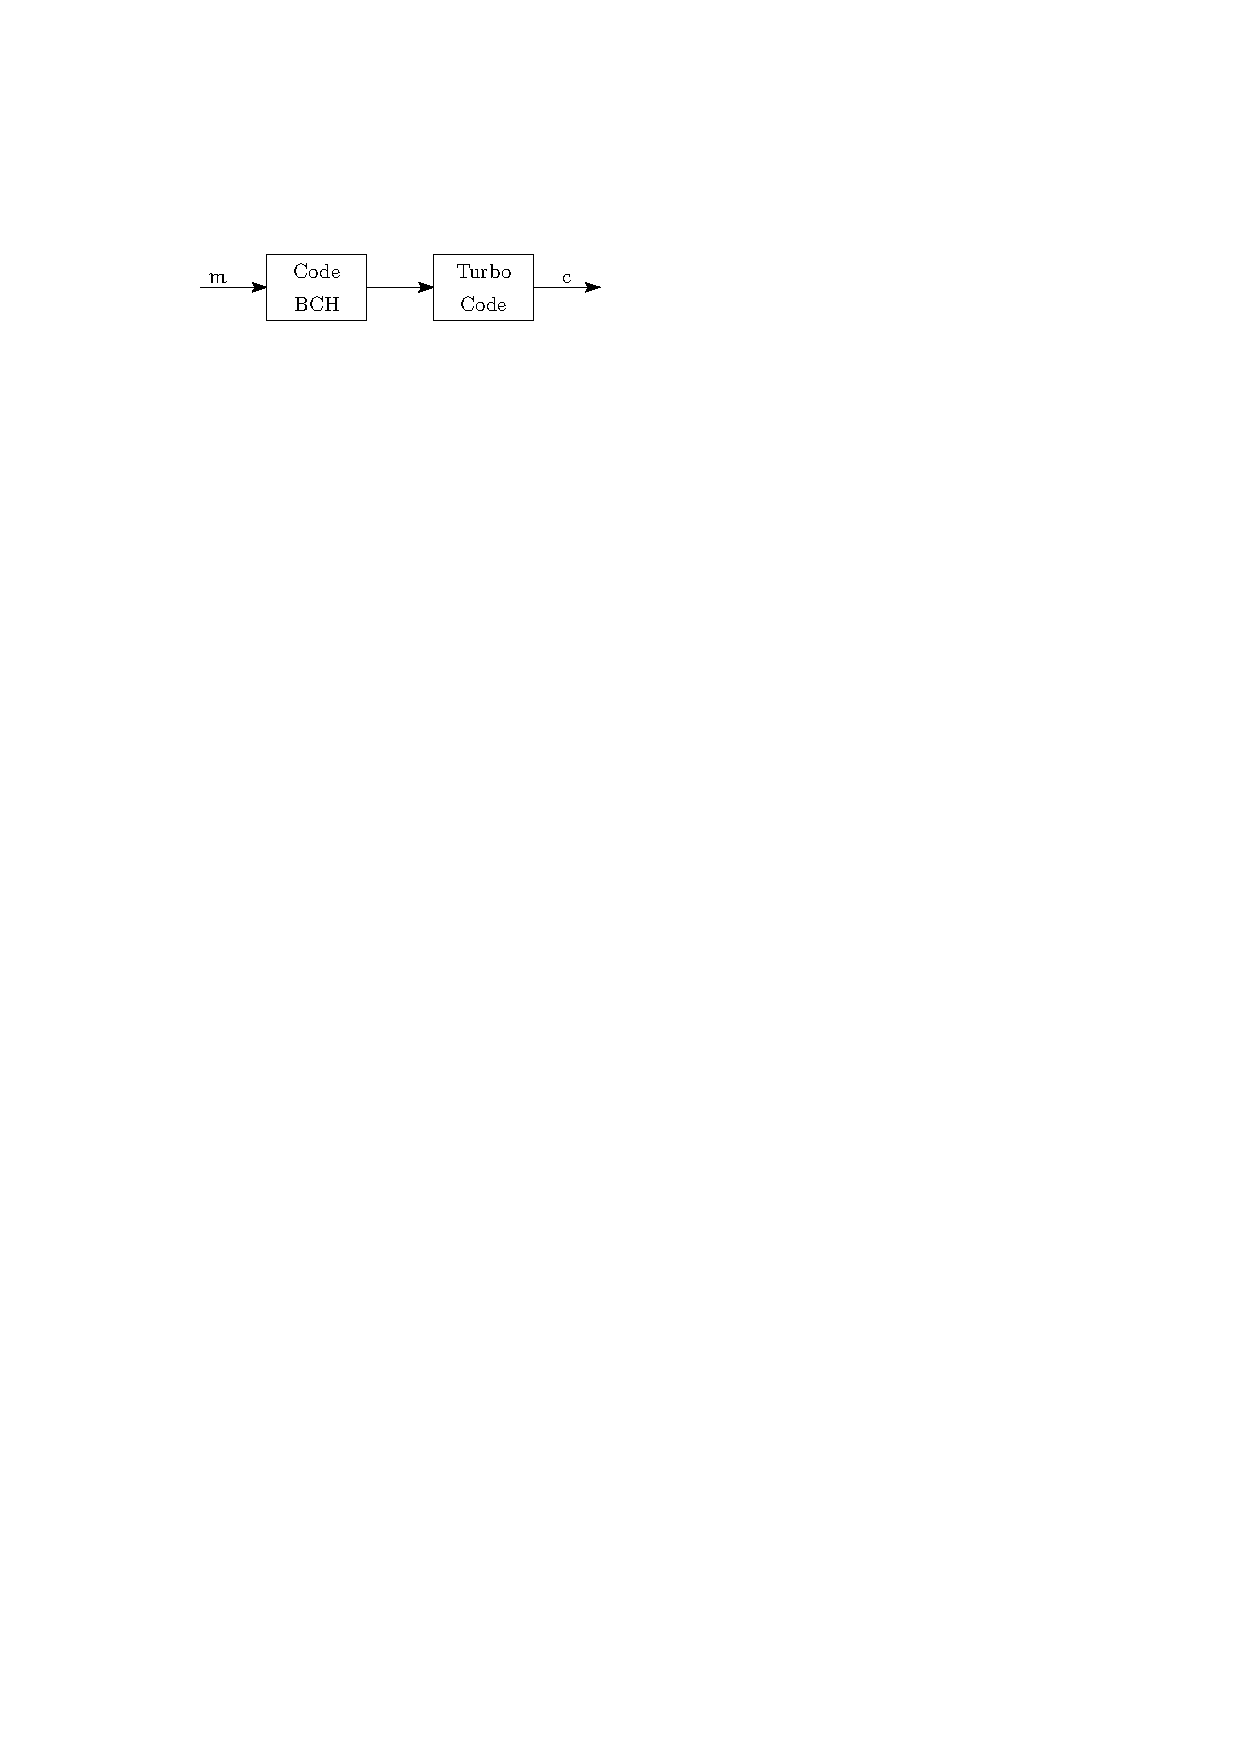
\includegraphics[]{main/ch1_fig/abaiss/bch.pdf}
	\end{center}
	\caption{Concaténation série d'un code BCH et d'un turbo code \label{fig:bchc}}
\end{figure}

\paragraph{Code RSC de rendement 1}
Le principe d'une concaténation basée sur un tel code est d'encoder partiellement soit l'information redondante provenant des codeurs élémentaires soit l'information systématique avant de la fournir aux codeurs élémentaires.

Le première forme de concaténation est nommée turbo codes 3D. Ces derniers ont été présentés par Berrou \textit{et al.} en 2007 \cite{TC3D_1}, puis analysés successivement dans \cite{TC3D_2} et \cite{TC3D_3}.
La forme est nommée quant à elle turbo code pré-codé. Leur proposition remonte à 2011 \cite{precoded}. Leur structure a été modifiée puis optimisée dans \cite{precoding}. Les codeurs associés sont présentés en Figure \ref{fig:t3d}.

Que ce soit pour les turbo codes 3D ou les turbo codes pré-codés, l'utilisation d'un code RSC de rendement 1 permet de ne pas modifier le rendement global du schéma de codage. Cependant, plus la part d'information 
traitée par ce codeur additionnel est importante, plus la convergence est retardée et plus la distance minimale est augmentée. Ainsi, un compromis peut être trouvé suivant les performances visées. 

Dans les deux cas, trois décodeurs SISO doivent échanger mutuellement de l'information. La complexité calculatoire du décodage augmente de façon notable. Dans \cite{TC3D_2}, une hausse de la complexité calculatoire du décodeur  d'environ $10\%$ est estimée. De plus, la latence de décodage augmente puisqu'une itération de décodage correspond dorénavant à l'activation successive des 3 décodeurs SISO.

\begin{figure}[tb]
  \begin{center}
    \subfloat[Turbo code 3D]{
      \includegraphics[width=0.45\textwidth]{main/ch1_fig/abaiss/t3d.pdf}
      \label{sub:t3d}
                         }
    \subfloat[Turbo code pré-codé]{
      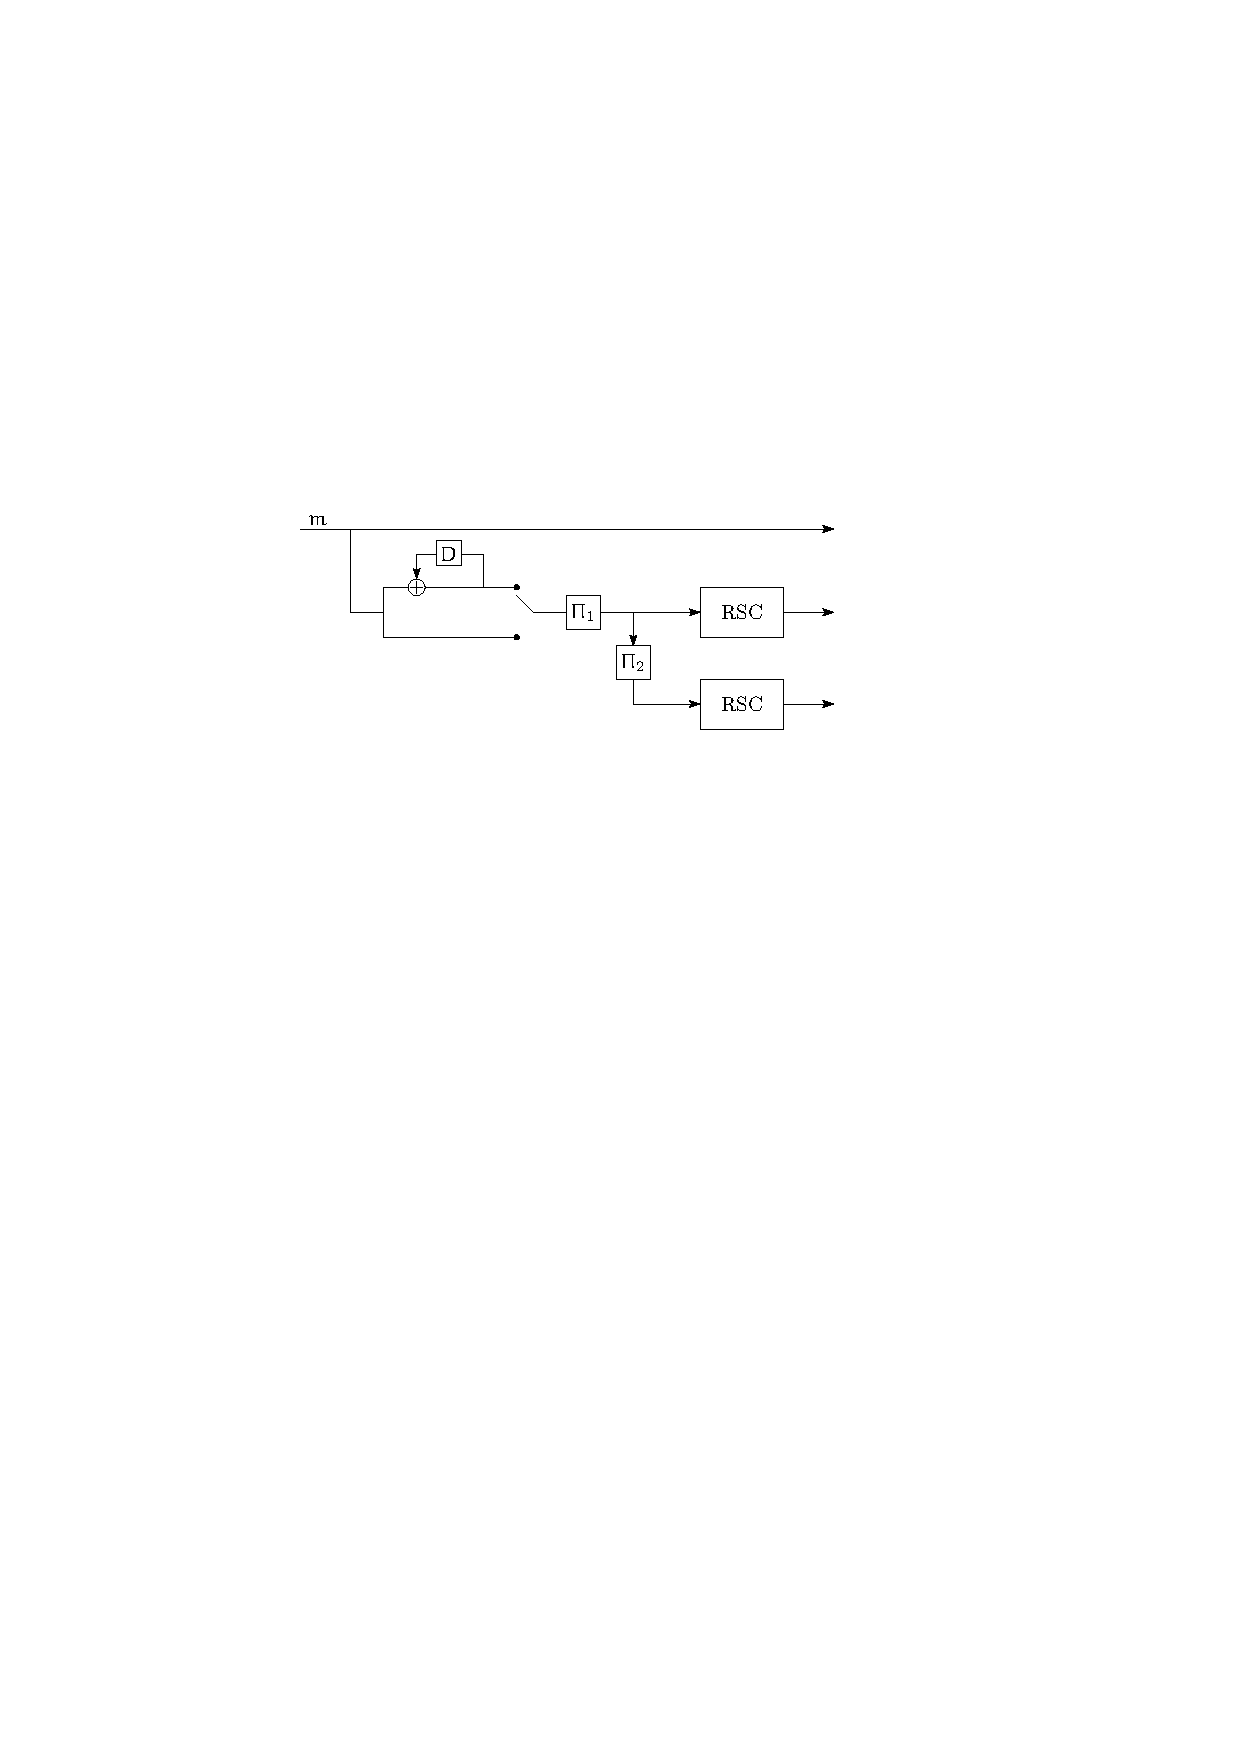
\includegraphics[width=0.45\textwidth]{main/ch1_fig/abaiss/precod.pdf}
      \label{sub:pre}
                         }
    \caption{Concaténation d'un turbo code et d'un RSC de rendement 1}
    \label{fig:t3d}
  \end{center}
\end{figure}

\paragraph{Code CRC}
La troisième concaténation utilise des codes détecteurs d'erreurs CRC. La concaténation série d'un tel code avec un turbo code est présenté en Figure \ref{fig:crc}. Cette famille de code possède un pouvoir de détection important. Ainsi, ce type de détecteur est souvent défini dans les standards employant des turbo codes. Par exemple, dans le standard LTE, ils permettent l'utilisation de demandes de renvoi automatique (ARQ). Dans ce cas, lorsque le récepteur détecte une erreur de transmission, il peut demander une retransmission des données. L'ARQ permet une amélioration de la qualité de service. D'autre part, les codes CRC peuvent aussi permettre d'arrêter le processus de décodage itératif dès lors que le turbo décodeur a convergé vers le bon mot de code. Des analyses comme dans \cite{detectionCRC} ont été menées afin de déterminer les probabilités d'erreurs non détectées et de fausse alerte lorsque qu'une détection CRC est effectuée au cours du processus itératif. 

Dans un but d'améliorer les performances de décodage, les codes CRC ont été utilisé de diverses manières. Celles-ci sont maintenant présentées.

\begin{figure}[b]
	\begin{center}
	\includegraphics[]{main/ch1_fig/abaiss/crc.pdf}
	\end{center}
	\caption{Concaténation série d'un code CRC et d'un turbo code \label{fig:crc}}
\end{figure}


\subparagraph{Décodage par liste} Cette famille de décodage a été pensée des la fin des années 50 indépendamment par Elias et Wozencraft \cite{elias1957list,wozencraft1958list}. Dans le cadre des codes convolutifs, son principe est de fournir les $\cal{L}$ séquences les plus probables correspondant à des chemins dans le treillis. Ces $\cal{L}$ séquences peuvent être obtenues grâce à l'algorithme de Viterbi par liste (LVA) selon une approche parallèle ou une approche séquentielle \cite{lva}. Plus récemment, une dérivation de l'algorithme ML-APP permettant d'obtenir $\cal{L}$ séquences a été proposée \cite{mlla}.
Dans le cadre du décodage de turbo codes par liste, trois principales approches peuvent être appliquées :
\begin{enumerate}
	\item \textbf{Intersection de liste : } Chacun des codes constituants est décodé selon un algorithme pat liste. Dès que l'intersection des deux ensembles de liste consiste en une seule séquence, le décodage s'arrête. Cette séquence est alors la sortie du décodeur \cite{sadowPair}. 
	\item \textbf{LVA post turbo : }  Le LVA peut aussi être réalisé en dehors du processus itératif usuel. Dans ce cas, il est exécuté après chaque itération ou à la fin du processus \cite{narayaList}. Les informations \textit{a posteriori} du turbo décodeur servent alors d'informations \textit{a priori} pour le LVA. Afin de déterminer la bonne séquence parmi les $\cal{L}$ séquences obtenues, un code détecteur d'erreurs est utilisé. Grâce à cette technique des gains notables, de l'ordre d'un facteur dix avec une liste de taille trois dans le plancher d'erreur, sont obtenus.
	\item \textbf{LVA pré turbo : } Le décodage liste peut aussi être appliqué avant le processus itératif. Il doit alors fournir $\cal{L}$ séquences distinctes de sorties souples qui seront utilisées en tant qu'information \textit{a priori} par $\cal{L}$ turbo décodeurs distincts. A nouveau, l'identification de la bonne séquence est réalisée par un code détecteur d'erreurs. Cette méthode propose des gains aussi bien dans la zone de convergence que dans le plancher d'erreur, mais possède un surcoût calculatoire important \cite{newList}. Ces gains représentent un facteur cinq pour de petites tailles de trame avec une liste de taille 16.
\end{enumerate}

Les décodeurs associés à ces différentes utilisations du LVA sont récapitulés en Figure \ref{fig:lva}. 


\begin{figure}[tb]
  \begin{center}
    \subfloat[Intersection de listes]{
      \includegraphics[width=0.45\textwidth]{main/ch1_fig/abaiss/lva_pll.pdf}
      \label{sub:lva1}}\\[1.5em] 
    \subfloat[LVA post turbo]{
      \includegraphics[width=0.5\textwidth]{main/ch1_fig/abaiss/lva_post.pdf}
      \label{sub:lva2}}\\[1.5em] 
    \subfloat[LVA pré turbo]{
      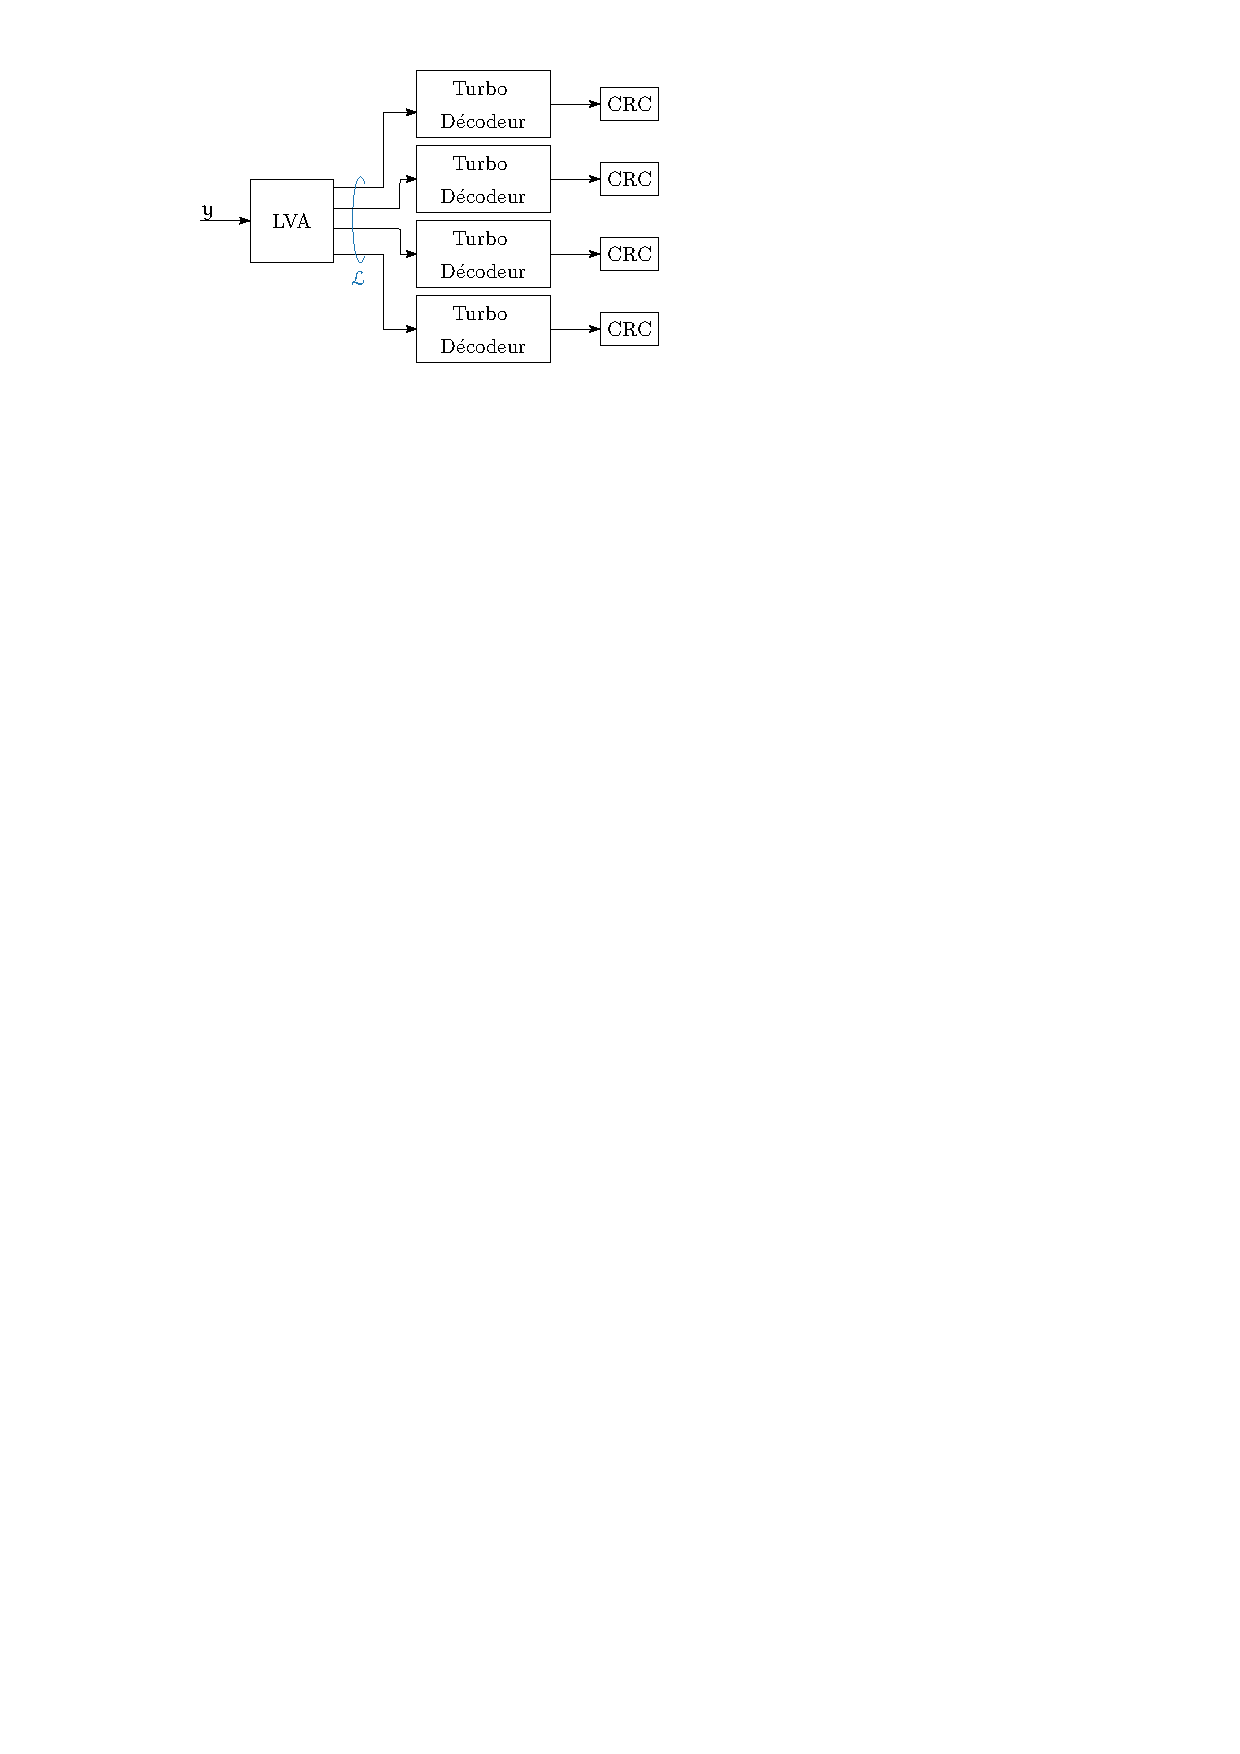
\includegraphics[width=0.5\textwidth]{main/ch1_fig/abaiss/lva_pre.pdf}
      \label{sub:lva3}}
    \caption{Décodeur utilisant l’algorithme de Viterbi par liste}
    \label{fig:lva}
  \end{center}
\end{figure}

\subparagraph{Décodage utilisant le décodage par statistiques ordonnées (OSD)} Des approches utilisant un tel décodage ont été proposées pour les turbo codes \cite{osdAided}. Le principe réside dans le fait d'appliquer l'OSD \cite{osd} de rang 1 après chaque itération de turbo décodage ou après le processus itératif. Une présentation schématique de ce principe est donné en Figure \ref{fig:osd}. Le décodage OSD se base sur la matrice génératrice du code. Celle-ci est permutée selon la fiabilité des informations. Grâce à une élimination Gaussienne et en inversant les décisions dures du décodeur turbo, $K$ mots sont identifiés. Finalement, le bon mot est sélectionné à l'aide d'un code détecteur d'erreurs. D'importants gains sont obtenus dans la zone de convergence pour de petites tailles de trame et de hauts rendements.  
Cette méthode a été étendue en considérant la matrice globale de la concaténation série du code CRC et du turbo code dans \cite{osdCrcAided}. Dans ce cas, le code CRC perd son pouvoir de détection mais les performances de décodage sont améliorées car la distance minimale du code concaténé est exploitée. Cependant, la complexité calculatoire de cette méthode est telle que seuls des décodages de trame de petite taille peuvent être envisagés.

\begin{figure}[tb]
\begin{center}
	\includegraphics[]{main/ch1_fig/abaiss/osd.pdf}
	\end{center}
	\caption{Décodage associant un turbo code et un décodeur OSD \label{fig:osd}}
\end{figure}

\subparagraph{Multiples turbo décodages} Cette méthode a été présentée par Crozier et Ould-Cheikh-Mouhamedou dans \cite{cim} puis reformulé dans \cite{fsm}. Son principe est le suivant. Si, à la fin du processus itératif, le décodeur n'a pas convergé vers le bon mot de code, les valeurs absolues des informations \textit{a posteriori} sont triées par ordre croissant. La valeur de l'information systématique correspondant à la position la moins fiable est alors forcée à une valeur supérieure à celle de la distance minimale du code. Un nouveau turbo décodage itératif est alors effectué. Le résultat est vérifié grâce à un code détecteur d'erreurs. Si le bon mot n'a pas été identifié, alors, la seconde position la moins fiable est forcée à une valeur supérieure à la distance minimale du code, tout en ayant remis la position la moins fiable à sa valeur originelle. Un nouveau turbo décodage itératif est alors effectué. Ce processus est répété jusqu'à ce qu'un nombre prédéfini de positions testées soit atteint ou jusqu'à ce que le code détecteur d'erreurs valide le mot courant.

Dans le cadre des turbo codes double binaires, les quatre possibilités de valeurs pour le couple $(A_i,B_i)$ sont considérées. Les performances de décodage sont améliorées à la fois dans la zone de convergence et au niveau du plancher d'erreur mais ce au prix, 
%d'une multiplication de la complexité calculatoire par le nombre de positions examinées. 
d'une multiplication par $4\times L$ de la complexité calculatoire avec $L$ le nombre de positions examinées.

Cette technique a été étendue par Pfletschinger dans \cite{pflet}. Cette fois toutes les informations provenant du canal sont considérées pour être fixées à une valeur supérieure à celle de la distance minimale du code. Ainsi, $N$ turbo décodages successifs peuvent être nécessaires. Afin d'obtenir les meilleures performances de décodage, un algorithme LVA est conjointement employé. Cependant, bien que cette méthode présente les meilleures performances de décodage, elle ne peut être considérée dans un contexte temps réel du fait de sa latence d'exécution et de la complexité calculatoire résultante.

\subsubsection{Récapitulatif des différentes méthodes d'abaissement du plancher d'erreur}
Dans cette section, différentes méthodes d'abaissement du plancher d'erreur sont récapitulées et comparées en terme de gains de décodage et de complexité de décodage. Une synthèse de cette comparaison est fournie dans le tableau \ref{tab:recap}.

Bien évidemment, toutes ces méthodes permettent d'abaisser le plancher d'erreur. De plus, les techniques utilisant l'OSD ou le turbo décodage multiple proposent des gains aussi dans la zone de convergence. Cependant leurs complexités calculatoires les excluent d'applications sous forte contrainte d'exécution. 

La concaténation avec un code BCH propose des gains intéressants dans la zone du plancher d'erreur tout en introduisant une complexité calculatoire modérée. Néanmoins, il est nécessaire d'ajouter des informations redondante (provenant du code BCH). Ceci implique une modification du rendement du code et donc un retard sur le seuil de convergence. 
En revanche, l'utilisation d'un code RSC de rendement 1 ne possède pas cet inconvénient mais nécessite cependant aussi de modifier le schéma de codage. Cette approche ne peut donc être utilisée dans des contextes déjà standardisés. De plus, le troisième SISO impacte négativement la complexité calculatoire et la latence du décodeur.

Finalement, les approches basées sur un décodage LVA successif au turbo décodage possèdent l'avantage de nécessiter uniquement l'adjonction d'un code CRC au turbo code. Des gains de performance sont observés dans le plancher d'erreur mais la complexité calculatoire ajoutée n'est pas négligeable.

\begin{table}[tb]
\centering
\caption{Synthèse des différentes méthodes améliorant les performances de décodage}
\label{tab:recap}
\resizebox{\textwidth}{!}{%
\begin{tabular}{rlllll}
\toprule
                  & BCH & RSC-1 & List Decoder & OSD & Décodages multiples\\
                  \cmidrule(l){2-2}\cmidrule(l){3-3}\cmidrule(l){4-4}\cmidrule(l){5-5}\cmidrule(l){6-6}
\textbf{Redondance ajoutée}         & Oui  & Non & CRC & CRC & CRC \\
\textbf{Localisation des gains}     & Plancher & Plancher & Plancher & Convergence et plancher & Convergence et plancher \\
\textbf{Complexité}                 & \thumbsup & \thumbsmid & \thumbsmid & \thumbsdown  & \thumbsdown \\
\bottomrule
\end{tabular}}
\end{table}

\section{Conclusion}
Dans ce premier chapitre, les notions permettant d'aborder le codage canal ont été successivement introduites. Puis, la construction, le décodage et les performances des turbo codes ont été détaillés. Des outils permettant d'estimer les performances d'un turbo code sur le canal BI-AWGN ont été présentés. Finalement, plusieurs méthodes permettant d'améliorer les performances de décodage des turbo codes ont été rapportées. Dans le cadre de turbo codes déjà standardisés, seules des méthodes appliquées au processus de décodage peuvent être employées. Or, comme le décodage des turbo codes est sous optimal, des optimisations doivent exister. Il est aussi à noter que de nombreux standards de communications numériques présentent un code CRC concaténé avec le turbo code. Ceci permet d'envisager une plus grande diversité de décodage. Pour l'ensemble de ces raisons, dans le chapitre suivant, afin d'améliorer les performances de décodage, des techniques de décodage tirant parti des oscillations au sein du turbo décodeur sont détaillées. 